% Lines starting with a percent sign (%) are comments. LaTeX will 
% not process those lines. Similarly, everything after a percent 
% sign in a line is considered a comment. To produce a percent sign
% in the output, write \% (backslash followed by the percent sign). 
% ==================================================================
% Usage instructions:
% ------------------------------------------------------------------
% The file is heavily commented so that you know what the various
% commands do. Feel free to remove any comments you don't need from
% your own copy. When redistributing the example thesis file, please
% retain all the comments for the benefit of other thesis writers! 
% ==================================================================
% Compilation instructions: 
% ------------------------------------------------------------------
% Use pdflatex to compile! Input images are expected as PDF files.
% Example compilation:
% ------------------------------------------------------------------
% > pdflatex thesis-example.tex
% > bibtex thesis-example
% > pdflatex thesis-example.tex
% > pdflatex thesis-example.tex
% ------------------------------------------------------------------
% You need to run pdflatex multiple times so that all the cross-references
% are fixed. pdflatex will tell you if you need to re-run it (a warning
% will be issued)  
% ------------------------------------------------------------------
% Compilation has been tested to work in ukk.cs.hut.fi and kosh.hut.fi
% - if you have problems of missing .sty -files, then the local LaTeX
% For example, when compiling in vipunen.hut.fi, you get an error that
% tikz.sty is missing - in this case you must either compile somewhere
% else, or you cannot use TikZ graphics in your thesis and must therefore
% remove or comment out the tikz package and all the tikz definitions. 
% ------------------------------------------------------------------
 
% General information
% ==================================================================
% Package documentation:
% 
% The comments often refer to package documentation. (Almost) all LaTeX
% packages have documentation accompanying them, so you can read the
% package documentation for further information. When a package 'xxx' is
% installed to your local LaTeX environment (the document compiles
% when you have \usepackage{xxx} and LaTeX does not complain), you can 
% find the documentation somewhere in the local LaTeX texmf directory
% hierarchy. In ukk.cs.hut.fi, this is /usr/texlive/2008/texmf-dist,
% and the documentation for the titlesec package (for example) can be 
% found at /usr/texlive/2008/texmf-dist/doc/latex/titlesec/titlesec.pdf.
% Most often the documentation is located as a PDF file in 
% /usr/texlive/2008/texmf-dist/doc/latex/xxx, where xxx is the package name; 
% however, documentation for TikZ is in
% /usr/texlive/2008/texmf-dist/doc/latex/generic/pgf/pgfmanual.pdf
% (this is because TikZ is a front-end for PGF, which is meant to be a 
% generic portable graphics format for LaTeX).
% You can try to look for the package manual using the ``find'' shell
% command in Linux machines; the find databases are up-to-date at least
% in ukk.cs.hut.fi. Just type ``find xxx'', where xxx is the package
% name, and you should find a documentation file.
% Note that in some packages, the documentation is in the DVI file
% format. In this case, you can copy the DVI file to your home directory,
% and convert it to PDF with the dvipdfm command (or you can read the
% DVI file directly with a DVI viewer).
% 
% If you can't find the documentation for a package, just try Googling
% for ``latex packagename''; most often you can get a direct link to the
% package manual in PDF format.
% ------------------------------------------------------------------


% Document class for the thesis is report
% ------------------------------------------------------------------
% You can change this but do so at your own risk - it may break other things.
% Note that the option pdftext is used for pdflatex; there is no
% pdflatex option. 
% ------------------------------------------------------------------
\documentclass[12pt,a4paper,oneside,pdftex]{report}

% The input files (tex files) are encoded with the latin-1 encoding 
% (ISO-8859-1 works). Change the latin1-option if you use UTF8 
% (at some point LaTeX did not work with UTF8, but I'm not sure
% what the current situation is) 
\usepackage[latin1]{inputenc}
% OT1 font encoding seems to work better than T1. Check the rendered
% PDF file to see if the fonts are encoded properly as vectors (instead
% of rendered bitmaps). You can do this by zooming very close to any letter 
% - if the letter is shown pixelated, you should change this setting 
% (try commenting out the entire line, for example).  
\usepackage[OT1]{fontenc}
% The babel package provides hyphenating instructions for LaTeX. Give
% the languages you wish to use in your thesis as options to the babel
% package (as shown below). You can remove any language you are not
% going to use.
% Examples of valid language codes: english (or USenglish), british, 
% finnish, swedish; and so on.
\usepackage[english]{babel}


% Font selection
% ------------------------------------------------------------------
% The default LaTeX font is a very good font for rendering your 
% thesis. It is a very professional font, which will always be 
% accepted. 
% If you, however, wish to spicen up your thesis, you can try out
% these font variants by uncommenting one of the following lines
% (or by finding another font package). The fonts shown here are 
% all fonts that you could use in your thesis (not too silly). 
% Changing the font causes the layouts to shift a bit; you many
% need to manually adjust some layouts. Check the warning messages
% LaTeX gives you.
% ------------------------------------------------------------------
% To find another font, check out the font catalogue from
% http://www.tug.dk/FontCatalogue/mathfonts.html
% This link points to the list of fonts that support maths, but
% that's a fairly important point for master's theses.
% ------------------------------------------------------------------
% <rant>
% Remember, there is no excuse to use Comic Sans, ever, in any
% situation! (Well, maybe in speech bubbles in comics, but there 
% are better options for those too)
% </rant>

% \usepackage{palatino}
% \usepackage{tgpagella}



% Optional packages
% ------------------------------------------------------------------
% Select those packages that you need for your thesis. You may delete
% or comment the rest.

% Natbib allows you to select the format of the bibliography references.
% The first example uses numbered citations: 
\usepackage[square,sort&compress,numbers]{natbib}
% The second example uses author-year citations.
% If you use author-year citations, change the bibliography style (below); 
% acm style does not work with author-year citations.
% Also, you should use \citet (cite in text) when you wish to refer
% to the author directly (\citet{blaablaa} said blaa blaa), and 
% \citep when you wish to refer similarly than with numbered citations
% (It has been said that blaa blaa~\citep{blaablaa}).
% \usepackage[square]{natbib}

% The alltt package provides an all-teletype environment that acts
% like verbatim but you can use LaTeX commands in it. Uncomment if 
% you want to use this environment. 
% \usepackage{alltt}

% The eurosym package provides a euro symbol. Use with \euro{}
\usepackage{eurosym} 

% Verbatim provides a standard teletype environment that renderes
% the text exactly as written in the tex file. Useful for code
% snippets (although you can also use the listings package to get
% automatic code formatting). 
\usepackage{verbatim}

% The listing package provides automatic code formatting utilities
% so that you can copy-paste code examples and have them rendered
% nicely. See the package documentation for details.
% \usepackage{listings}

% The fancuvrb package provides fancier verbatim environments 
% (you can, for example, put borders around the verbatim text area
% and so on). See package for details.
% \usepackage{fancyvrb}

% Supertabular provides a tabular environment that can span multiple 
% pages. 
%\usepackage{supertabular}
% Longtable provides a tabular environment that can span multiple 
% pages. This is used in the example acronyms file. 
\usepackage{longtable}

% The fancyhdr package allows you to set your the page headers 
% manually, and allows you to add separator lines and so on. 
% Check the package documentation. 
% \usepackage{fancyhdr}

% Subfigure package allows you to use subfigures (i.e. many subfigures
% within one figure environment). These can have different labels and
% they are numbered automatically. Check the package documentation. 
\usepackage{subfigure}

% The titlesec package can be used to alter the look of the titles 
% of sections, chapters, and so on. This example uses the ``medium'' 
% package option which sets the titles to a medium size, making them
% a bit smaller than what is the default. You can fine-tune the 
% title fonts and sizes by using the package options. See the package
% documentation.
\usepackage[medium]{titlesec}
\usepackage{etoolbox}
\makeatletter
\patchcmd{\ttlh@hang}{\parindent\z@}{\parindent\z@\leavevmode}{}{}
\patchcmd{\ttlh@hang}{\noindent}{}{}{}
\makeatother

% The TikZ package allows you to create professional technical figures.
% The learning curve is quite steep, but it is definitely worth it if 
% you wish to have really good-looking technical figures. 
\usepackage{tikz}
% You also need to specify which TikZ libraries you use
\usetikzlibrary{positioning}
\usetikzlibrary{calc}
\usetikzlibrary{arrows}
\usetikzlibrary{decorations.pathmorphing,decorations.markings}
\usetikzlibrary{shapes}
\usetikzlibrary{patterns}


% The aalto-thesis package provides typesetting instructions for the
% standard master's thesis parts (abstracts, front page, and so on)
% Load this package second-to-last, just before the hyperref package.
% Options that you can use: 
%   mydraft - renders the thesis in draft mode. 
%             Do not use for the final version. 
%   doublenumbering - [optional] number the first pages of the thesis
%                     with roman numerals (i, ii, iii, ...); and start
%                     arabic numbering (1, 2, 3, ...) only on the 
%                     first page of the first chapter
%   twoinstructors  - changes the title of instructors to plural form
%   twosupervisors  - changes the title of supervisors to plural form
%\usepackage[mydraft,twosupervisors]{aalto-thesis}
\usepackage[mydraft,doublenumbering]{aalto-thesis}
%\usepackage[mydraft]{aalto-thesis}


% Hyperref
% ------------------------------------------------------------------
% Hyperref creates links from URLs, for references, and creates a
% TOC in the PDF file.
% This package must be the last one you include, because it has
% compatibility issues with many other packages and it fixes
% those issues when it is loaded.   
\RequirePackage[pdftex]{hyperref}
% Setup hyperref so that links are clickable but do not look 
% different
\hypersetup{colorlinks=false,raiselinks=false,breaklinks=true}
\hypersetup{pdfborder={0 0 0}}
\hypersetup{bookmarksnumbered=true}
% The following line suggests the PDF reader that it should show the 
% first level of bookmarks opened in the hierarchical bookmark view. 
\hypersetup{bookmarksopen=true,bookmarksopenlevel=1}
% Hyperref can also set up the PDF metadata fields. These are
% set a bit later on, after the thesis setup.   


% Thesis setup
% ==================================================================
% Change these to fit your own thesis.
% \COMMAND always refers to the English version;
% \FCOMMAND refers to the Finnish version; and
% \SCOMMAND refers to the Swedish version.
% You may comment/remove those language variants that you do not use
% (but then you must not include the abstracts for that language)
% ------------------------------------------------------------------
% If you do not find the command for a text that is shown in the cover page or
% in the abstract texts, check the aalto-thesis.sty file and locate the text
% from there. 
% All the texts are configured in language-specific blocks (lots of commands
% that look like this: \renewcommand{\ATCITY}{Espoo}.
% You can just fix the texts there. Just remember to check all the language
% variants you use (they are all there in the same place). 
% ------------------------------------------------------------------
\newcommand{\TITLE}{Contracting Service For Industrial Internet}
%\newcommand{\FTITLE}{Ohjelmistoprosessit m�nteille:}
%\newcommand{\STITLE}{Den stora stygga vargen:}
\newcommand{\SUBTITLE}{Re-inventing the Wheel}
%\newcommand{\FSUBTITLE}{Uusi organisaatio, uudet py�r�t}
%\newcommand{\SSUBTITLE}{Lilla Vargens universum}
\newcommand{\DATE}{June 18, 2011}
%\newcommand{\FDATE}{18. kes�kuuta 2011}
%\newcommand{\SDATE}{Den 18 Juni 2011}

% Supervisors and instructors
% ------------------------------------------------------------------
% If you have two supervisors, write both names here, separate them with a 
% double-backslash (see below for an example)
% Also remember to add the package option ``twosupervisors'' or
% ``twoinstructors'' to the aalto-thesis package so that the titles are in
% plural.
% Example of one supervisor:
\newcommand{\SUPERVISOR}{Professor Petri Vuorimaa}
%\newcommand{\FSUPERVISOR}{Professori Antti Yl�-J��ski}
%\newcommand{\SSUPERVISOR}{Professor Antti Yl�-J��ski}
% Example of twosupervisors:
%\newcommand{\SUPERVISOR}{Professor Antti Yl�-J��ski\\
%  Professor Pekka Perustieteilij�}
%\newcommand{\FSUPERVISOR}{Professori Antti Yl�-J��ski\\
%  Professori Pekka Perustieteilij�}
%\newcommand{\SSUPERVISOR}{Professor Antti Yl�-J��ski\\
%  Professor Pekka Perustieteilij�}

% If you have only one instructor, just write one name here
\newcommand{\INSTRUCTOR}{Instructor?}
%\newcommand{\FINSTRUCTOR}{Diplomi-insin��ri Olli Ohjaaja}
%\newcommand{\SINSTRUCTOR}{Diplomingenj�r Olli Ohjaaja}
% If you have two instructors, separate them with \\ to create linefeeds
% \newcommand{\INSTRUCTOR}{Olli Ohjaaja M.Sc. (Tech.)\\
%  Elli Opas M.Sc. (Tech)}
%\newcommand{\FINSTRUCTOR}{Diplomi-insin��ri Olli Ohjaaja\\
%  Diplomi-insin��ri Elli Opas}
%\newcommand{\SINSTRUCTOR}{Diplomingenj�r Olli Ohjaaja\\
%  Diplomingenj�r Elli Opas}

% If you have two supervisors, it is common to write the schools
% of the supervisors in the cover page. If the following command is defined,
% then the supervisor names shown here are printed in the cover page. Otherwise,
% the supervisor names defined above are used.
\newcommand{\COVERSUPERVISOR}{Professor Petri Vuorimaa, Aalto University}

% The same option is for the instructors, if you have multiple instructors.
% \newcommand{\COVERINSTRUCTOR}{Olli Ohjaaja M.Sc. (Tech.), Aalto University\\
%  Elli Opas M.Sc. (Tech), Aalto SCI}


% Other stuff
% ------------------------------------------------------------------
\newcommand{\PROFESSORSHIP}{Hypermedia}
%\newcommand{\FPROFESSORSHIP}{Tietoliikenneohjelmistot}
%\newcommand{\SPROFESSORSHIP}{Datakommunikationsprogram}
% Professorship code is the same in all languages
\newcommand{\PROFCODE}{T-110}
\newcommand{\KEYWORDS}{ocean, sea, marine, ocean mammal, marine mammal, whales,
cetaceans, dolphins, porpoises}
%\newcommand{\FKEYWORDS}{AEL, aineistot, aitta, akustiikka, Alankomaat,
%aluerakentaminen, Anttolanhovi, Arcada, ArchiCad, arkki}
%\newcommand{\SKEYWORDS}{oms�ttning, kassafl�de, v�rdepappersmarknadslagen,
%yrkesut�vare, intressef�retag, verifieringskedja}
\newcommand{\LANGUAGE}{English}
%\newcommand{\FLANGUAGE}{Englanti}
%\newcommand{\SLANGUAGE}{Engelska}

% Author is the same for all languages
\newcommand{\AUTHOR}{Relja Paunovic}


% Currently the English versions are used for the PDF file metadata
% Set the PDF title
\hypersetup{pdftitle={\TITLE\ \SUBTITLE}}
% Set the PDF author
\hypersetup{pdfauthor={\AUTHOR}}
% Set the PDF keywords
\hypersetup{pdfkeywords={\KEYWORDS}}
% Set the PDF subject
\hypersetup{pdfsubject={Master's Thesis}}


% Layout settings
% ------------------------------------------------------------------

% When you write in English, you should use the standard LaTeX 
% paragraph formatting: paragraphs are indented, and there is no 
% space between paragraphs.
% When writing in Finnish, we often use no indentation in the
% beginning of the paragraph, and there is some space between the 
% paragraphs. 

% If you write your thesis Finnish, uncomment these lines; if 
% you write in English, leave these lines commented! 
% \setlength{\parindent}{0pt}
% \setlength{\parskip}{1ex}

% Use this to control how much space there is between each line of text.
% 1 is normal (no extra space), 1.3 is about one-half more space, and
% 1.6 is about double line spacing.  
% \linespread{1} % This is the default
% \linespread{1.3}

% Bibliography style
% acm style gives you a basic reference style. It works only with numbered
% references.
\bibliographystyle{acm}
% Plainnat is a plain style that works with both numbered and name citations.
% \bibliographystyle{plainnat}


% Extra hyphenation settings
% ------------------------------------------------------------------
% You can list here all the files that are not hyphenated correctly.
% You can provide many \hyphenation commands and/or separate each word
% with a space inside a single command. Put hyphens in the places where
% a word can be hyphenated.
% Note that (by default) LaTeX will not hyphenate words that already
% have a hyphen in them (for example, if you write ``structure-modification 
% operation'', the word structure-modification will never be hyphenated).
% You need a special package to hyphenate those words.
\hyphenation{di-gi-taa-li-sta yksi-suun-tai-sta}



% The preamble ends here, and the document begins. 
% Place all formatting commands and such before this line.
% ------------------------------------------------------------------
\begin{document}
% This command adds a PDF bookmark to the cover page. You may leave
% it out if you don't like it...
\pdfbookmark[0]{Cover page}{bookmark.0.cover}
% This command is defined in aalto-thesis.sty. It controls the page 
% numbering based on whether the doublenumbering option is specified
\startcoverpage

% Cover page
% ------------------------------------------------------------------
% Options: finnish, english, and swedish
% These control in which language the cover-page information is shown
\coverpage{english}


% Abstracts
% ------------------------------------------------------------------
% Include an abstract in the language that the thesis is written in,
% and if your native language is Finnish or Swedish, one in that language.

% Abstract in English
% ------------------------------------------------------------------
\thesisabstract{english}{
A dissertation or thesis is a document submitted in support of candidature
for a degree or professional qualification presenting the author's research and
findings. In some countries/universities, the word thesis or a cognate is used
as part of a bachelor's or master's course, while dissertation is normally
applied to a doctorate, whilst, in others, the reverse is true.

\fixme{Abstract text goes here (and this is an example how to use fixme).} 
Fixme is a command that helps you identify parts of your thesis that still
require some work. When compiled in the custom \texttt{mydraft} mode, text
parts tagged with fixmes are shown in bold and with fixme tags around them. When
compiled in normal mode, the fixme-tagged text is shown normally (without
special formatting). The draft mode also causes the ``Draft'' text to appear on
the front page, alongside with the document compilation date. The custom
\texttt{mydraft} mode is selected by the \texttt{mydraft} option given for the
package \texttt{aalto-thesis}, near the top of the \texttt{thesis-example.tex}
file.

The thesis example file (\texttt{thesis-example.tex}), all the chapter content
files (\texttt{1introduction.tex} and so on), and the Aalto style file
(\texttt{aalto-thesis.sty}) are commented with explanations on how the Aalto
thesis works. The files also contain some examples on how to customize various
details of the thesis layout, and of course the example text works as an
example in itself. Please read the comments and the example text; that should
get you well on your way!}


% Acknowledgements
% ------------------------------------------------------------------
% Select the language you use in your acknowledgements
\selectlanguage{english}

% Uncomment this line if you wish acknoledgements to appear in the 
% table of contents
%\addcontentsline{toc}{chapter}{Acknowledgements}

% The star means that the chapter isn't numbered and does not 
% show up in the TOC
\chapter*{Acknowledgements}

I wish to thank all students who use \LaTeX\ for formatting their theses,
because theses formatted with \LaTeX\ are just so nice.

Thank you, and keep up the good work!
\vskip 10mm

\noindent Espoo, \DATE
\vskip 5mm
\noindent\AUTHOR

% Acronyms
% ------------------------------------------------------------------
% Use \cleardoublepage so that IF two-sided printing is used 
% (which is not often for masters theses), then the pages will still
% start correctly on the right-hand side.
\cleardoublepage
% Example acronyms are placed in a separate file, acronyms.tex
\addcontentsline{toc}{chapter}{Abbreviations and Acronyms}
\chapter*{Abbreviations and Acronyms}

% The longtable environment should break the table properly to multiple pages, 
% if needed

\noindent
\begin{longtable}{@{}p{0.25\textwidth}p{0.7\textwidth}@{}}
IOT & Internet Of Things \\
IIOT & Industrial Internet of Things \\
ETSI & European Telecommunications Standards Institute \\
M2M & Machine To Machine \\
GSCM2MTF & Global Standards Collaboration Machine-to-Machine Task Force (GSCM2MTF) \\
3GPP & 3rd Generation Partnership Project \\ 
ETSI & European Telecommunications Standards Institute \\
REST & Representational State Transfer \\
SCL & RESTful Service Capability Layer \\
OMA & Open Mobile Alliance \\
LWM2M & Light Weight Machine-to-Machine \\
CoAP & Constrained Application Protocol \\
DoS & Denial of Service \\  
FQDN & Fully Qualified Domain Name \\
CES & Customer Edge Switching \\

\end{longtable}


% Table of contents
% ------------------------------------------------------------------
\cleardoublepage
% This command adds a PDF bookmark that links to the contents.
% You can use \addcontentsline{} as well, but that also adds contents
% entry to the table of contents, which is kind of redundant.
% The text ``Contents'' is shown in the PDF bookmark. 
\pdfbookmark[0]{Contents}{bookmark.0.contents}
\tableofcontents

% List of tables
% ------------------------------------------------------------------
% You only need a list of tables for your thesis if you have very 
% many tables. If you do, uncomment the following two lines.
% \cleardoublepage
% \listoftables

% Table of figures
% ------------------------------------------------------------------
% You only need a list of figures for your thesis if you have very 
% many figures. If you do, uncomment the following two lines.
% \cleardoublepage
% \listoffigures

% The following label is used for counting the prelude pages
\label{pages-prelude}
\cleardoublepage

%%%%%%%%%%%%%%%%% The main content starts here %%%%%%%%%%%%%%%%%%%%%
% ------------------------------------------------------------------
% This command is defined in aalto-thesis.sty. It controls the page 
% numbering based on whether the doublenumbering option is specified
\startfirstchapter

% Add headings to pages (the chapter title is shown)
\pagestyle{headings}

% The contents of the thesis are separated to their own files.
% Edit the content in these files, rename them as necessary.
% ------------------------------------------------------------------
\chapter{Introduction}
\label{chapter:intro}

This is my master's thesis, and I am very proud of it.  Of course,
when I write my \emph{real} master's thesis, I will not use the
singular pronoun \emph{I}, but rather try to avoid referring to myself
and speak of the research \emph{we} have conducted---I rarely work
alone, after all.  Yet, both \emph{I} and \emph{we} are correct, and
it depends on the instructor and the supervisor (of course from you,
too), which one they would prefer. Anyway, the tense should be active,
and passive sentenses should be avoided (especially, writing sentences
where the subject is presented with by preposition), so often you
cannot avoid choosing between the pronouns. Life is strange, but there
you have it.

By the way, the preferred order of writing your master's thesis is
about the same as the outline of the thesis: you first discover your
problem and write about that, then you find out what methods you
should use and write about that.  Then you do your implementation, and
document that, and so on.  However, the abstract and introduction are
often easiest to write last.  This is because these really cover the
entire thesis, and there is no way you could know what to put in your
abstract before you have actually done your implementation and
evaluation. Rarely anyone write the thesis from the beginning to the
end just one time, but the writing is more like process, where every
piece of text is written at least twice. Be also prepared to delete
your own text. In the first phase, you can hide it into comments that
are started with \% but during the writing, the many comments should be
visible for your helpers, the instructor and supervisor.

The introduction in itself is rarely very long; two to five pages often
suffice.


\section{Problem statement}

Undergraduate students studying technical subjects do not consider typography
very interesting these days, and therefore the typographical quality of many
theses is unacceptably low. 
We plan to rectify this situation somewhat by providing a decent-quality
example thesis outline for students.
We expect that the typographical quality of the master's theses will
dramatically increase as the new thesis outline is taken into use.

\section{Helpful hints}

Read the information from the university master's thesis
pages~\cite{ThesisInstructions} before starting the thesis.  You
should also go through the thesis grading
instructions~\cite{ThesisGrading} together with your instructor and/or
supervisor in the beginning of your work.

\section{Structure of the Thesis}
\label{section:structure}

You should use transition in your text, meaning that you should help
the reader follow the thesis outline. Here, you tell what will be in
each chapter of your thesis. 



\chapter{Literature Review}
\label{chapter:background} 

In the following section, I will give overview about Internet of Things (IOT) and Industrial Internet of Things (IIOT), highlighting differences between them. Further, I will describe open issues in IIOT followed by standardization attempts and related work regarding security. At the end of this chapter, I will give a more detailed description of most notable standards, Light Weight Machine-to-Machine (LWM2M) and Web of Things at the end of this chapter followed by Policy Based Communications, which is the basis of this work.

\section{Internet of Things}

%Short introduction about IOT
Internet of things (IOT) is a relatively new concept gaining momentum since the start of this century. Although, first examples
of IOT date back as early as 1983 with an automated inventory system. IOT can be seen as an extension to Internet, with physical devices (such as sensors and actuators) communicating with each other and with humans creating an enormous network.

Nowadays, with the continuous decrease in cost of computational devices, 
we are able to produce powerful devices with communication abilities for a very low price. With the increase in number 
of devices that needs to be connected (some estimates show up to 75 billion connected devices by year 2025\footnote{https://www.statista.com/statistics/471264/iot-number-of-connected-devices-worldwide/}), issues regarding scalability, security, heterogeneity of devices, etc. have emerged. 

These issues are holding back the progress of IOT because it forces companies to create their own proprietary systems to fit their needs, which is only an option for
large companies with financial capabilities to do so. This leads to large number of systems designed for similar purposes but incompatible with each other (due to use of different protocols or architectures). Temporary solution for this problem is to introduce a middle-ware as proposed by \cite{Bandyopadhyay2011} that acts like a bridge between two systems, but this has scalability issues and with the rise of number of connected devices will soon be unacceptable. In order to tackle these issues, several standards have been proposed, most notably smartM2M, oneM2M and most recently LightweightM2M (LWM2M), which will be explained in ~\ref{section:Standardization}. None of these have yet become \emph{de facto} standard.

In the remainder of this section, differences between Industrial Internet of Things (IIOT) and IOT will be introduced followed by open issues of IOT and IIOT  in ~\ref{section:OpenIssues}.


\subsection{Industrial Internet of Things}

In IOT, a rough distinction is made between consumer and industrial IOT according to \cite{Bandyopadhyay2011}. Consumer IOT applications are aimed to make everyday life easier by saving time and money, such as smart locks, smart homes and wearable hearth monitors. On the other hand, industrial IOT (such as production, automation and intelligent computation systems) focuses on how smart machines, data analytics and networked sensors can improve services in business-to-business domain 
\cite{Palattella2016}. As an example, predictive maintenance can generate savings up to 12\% over scheduled repairs, leading to a 30\% reduction in maintenance cost and a 70\% cut in downtime from equipment breakdowns according to Accenture\footnote{https://www.accenture.com/us-en/insight-industrial-internet-of-things}.This usually implies extensive machine-to-machine (M2M) communication compared to consumer IOT, where in most cases real time guarantees are not required.

Generally, IIOT has stricter requirements regarding delay, security and general robustness compared to consumer IOT. This is because failures in these devices can have consequences on safety of people and environment. For example, in a factory setting, pressure sensor installed on an indoor crane can cause serious damage by failing to communicate about an obstruction.

\subsection{Open Issues}
\label{section:OpenIssues}
As previously mentioned, there are many issues surrounding IOT, most notably, lack of standards and security. These issues will be explained in the remainder of the section.

\subsubsection{Standardization}
\label{section:Standardization}

According to Global Standards Collaboration Machine-to-Machine Task Force (GSCM2MTF) there are more than 140 organizations involved in the M2M standardization process worldwide.  
This is a huge vertical fragmentation of IOT market, and it is a result of long history in Industrial use, starting from seventies with process control systems that continued to be used in todays process automation systems. As already mentioned, these systems are proprietary and are incompatible with each other.

In an attempt to resolve this fragmentation issue three notable initiatives stand out. SmartM2M is an initiative led by European Telecommunications Standards Institute (ETSI), it is based on RESTful Service Capability Layer (SCL) \cite{Alaya2014} which is available through open interfaces. Resource tree residing on SCL along with procedures for handling them is standardized following Representational State Transfer (REST) principles allowing technology agnostic way of accessing them. SmartM2M also defines security framework including  authentication, M2M service bootstrap, key agreement and establishment, and M2M service connection procedures, based on a key hierarchy of the M2M node\cite{ETSI1}. Unfortunately, it may have issues with scalability as pointed out by \cite{Grieco2014}, thus, making it unsuitable for IOT and IIOT. 

A follow up project was formed in order to resolve issues with SmartM2M, this time with a broader partnership. It is an international project started by seven telecom standards organizations: Association of Radio Industries and Businesses (ARIB) and Telecommunication Technology Committee (TTC), Japan; the Alliance for Telecommunications Industry Solutions (ATIS) and Telecommunications Industry Association (TIA), United States; the China Communications Standards Association (CCSA), China; the European Telecommunications Standards Institute (ETSI), Europe; and the Telecommunications Technology Association (TTA), Korea. This project is based on RESTfull design, same as SmartM2M, resource naming conventions same as SmartM2M and is grounded on horizontal service layer principle. Although, it relaxes the scalability constraints by using hierarchical organization of different actors in the system. With this improvement with respect to SmartM2M, it is a serious contester to became IOT standard, being already adopted by various companies according to \cite{Park2016}. Along with these improvements, it defines a security architecture in three layers: security functions, security environment abstraction and security environment.

Recently, a new standard has emerged from Open Mobile Alliance (OMA) targeting constrained devices named Light Weight Machine-to-Machine (LWM2M). It defines a fast deployable client-server specification while minimizing memory consumption and network overhead making it very appealing to IOT and IIOT devices. It provides device management and security work-flow for IOT applications in a very light weight manner. Recent results from \cite{Rao2015} show that memory footprint overheads on a client side protocol stack are no more than 6-9\%. 

Another standard has recently been announced by World-wide-web Consortium (W3C) named Web of Things (WOT). This standards aims to provide a middleware (presented as an abstraction layer) to connect different IOT platforms and protocols. Detailed description of LWM2M and WOT will be given in section ~\ref{section:NotableStandards} since they represent two best candidates for this work.


\subsubsection{Security and privacy}
%\fixme{Authentication, Data integrity, Privacy}

Devices in IOT generate, process and exchange vast amount of data that is safety-critical and/or private and they are subject to various attacks. Therefore, it is crucial to assure integrity of the devices code and data from malicious modifications \cite{Control2014}. In IIOT, following two requirements are crucial for security according to \cite{Sadeghi2015}. Availability is most important requirement, because it can lead to loss in productivity and consequently loss of revenue. This is particularly affected by denial of service (DoS) attacks and preventing any system failure that may result in physical damage or harm to humans, particularly affected by sabotage.

There are many security architectures for embedded IOT devices, although, majority of them are too complex for low-end devices. Solutions for low-end devices usually rely on physical (hardware) isolation of security-critical code and data from other software on same device. Examples of such architectures are SMART \cite{Smart}, SPM \cite{SPM}, SANCTUS \cite{Sanctus} and TrustLite \cite{TrustLite} but they all have major flaws. SMART does not allow code changes after deployment. SPM and SANCTUS have hardware assisted task isolation but they are non-interruptible, which violates real-time guarantees. TrustLite requires all software components to be loaded at boot time, which reduces flexibility. TyTAN \cite{Brasser} is the only work that provides secure loading of tasks at runtime, secure inter-process communication, local and remote attestation and real-time guarantees. 
\section{Notable standards}
\label{section:NotableStandards}

Following section will describe two most notable standards which were final candidates for this thesis. These standards come from Open Mobile Alliance and World-wide-web Consortium which are two biggest standardization bodies in mobile communications and Web respectively.

\subsection{Light Weight Machine to Machine (LWM2M)}
\label{section:LWM2M}

OMA has approved first version (V1.0) of LWM2M standard in February 2017, since it is a very recent specification not many implementations exist, although, number has been steadily increasing since then. Most notable implementation by \cite{Rao2015} focuses on client side architecture (residing on IOT devices).

LWM2M provides a light and secure communication interface with compact data model to enable device management and service for IOT (and IIOT) devices. It is a client-server architecture named OMA LWM2M Enabler. Enabler consists of LWM2M Server, which is a central point that takes care of the devices, assigning security keys, registering device capabilities and more. Another part of Enabler is LWM2M Client, which resides on a device and provides necessary information to the Server. Furthermore, it uses Constrained Application Protocol (COAP), instead of HTTP, which has a greatly reduced communication overhead making it ideal for constrained devices (or devices benefiting from efficient communication, as the case in IIOT) along with UDP/SMS transport bindings. Architecture of LWM2M is shown on Figure ~\ref{fig:LWM2MArchitecture}.

\begin{figure}[ht]
	\begin{center}
		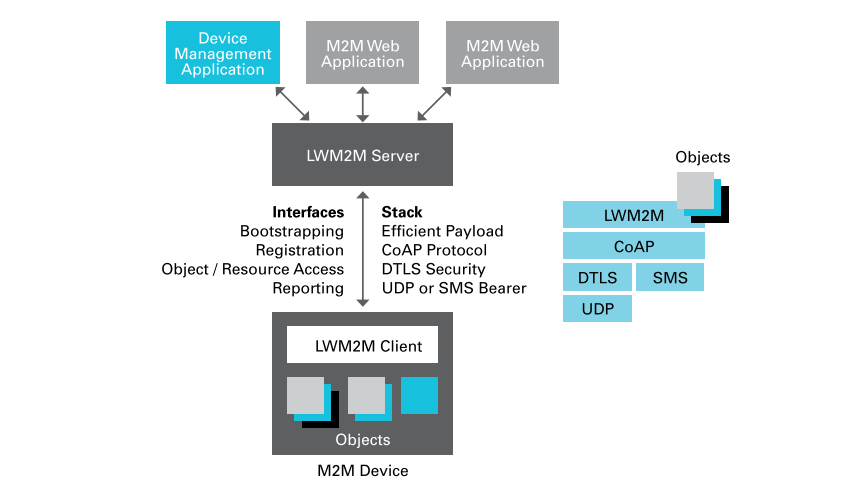
\includegraphics[width=\textwidth]{images/LWM2M-Architecture}
		\caption{LWM2M Architecture}
		\label{fig:LWM2MArchitecture}
	\end{center}
\end{figure}

The LWM2M Enabler defines the application layer communication protocol between Server and Client. It is separated into four logical interfaces, namely, Bootstrap, Device Discovery and Registration, Device Management and Service Enablement, and Information Reporting. Diagram showing interfaces and corresponding messages is illustrated in ~\ref{fig:LWM2MInterfaces}.

\begin{enumerate}
	\setlength{\itemsep}{1pt}
	\item Bootstrap: allows LWM2M Bootstrap server to manage keying, access control and to configure device for communication with the Server.
	\item Device Discovery and Registration: allows Server to discover devices and register their capabilities, e.g., which objects and how to access them does a device have.
	\item Device Management and Service Enablement: allows LWM2M Server to manage devices and provide M2M service by sending operations to devices and getting corresponding responses from them.
	\item Information Reporting: This is a core interface in LWM2M, which allows reporting of resource information. It can be triggered periodically, on events or on request.
\end{enumerate}

Communication model of LWM2M is based on CoAP methods similar to HTTP verbs GET, POST, PUT, DELETE to manipulate \emph{resources} on devices. Compared to HTTP, CoAP starts with only four bytes of overhead in binary encoded message and is easily translatable to HTTP. Unlike HTTP, CoAP messages are exchanged asynchronously between CoAP end-points over a datagram-oriented transport, in this case UDP.

In LWM2M Enabler, each individually addressable piece of information is called a Resource and groups of Resources are logically organized into Objects. For example, predefined object \emph{Location} contains all resources needed for locating the device. Full list of existing objects can be found at OMA registry \footnote{http://www.openmobilealliance.org/wp/OMNA/LwM2M/LwM2MRegistry.html}.

\begin{figure}[ht]
	\begin{center}
		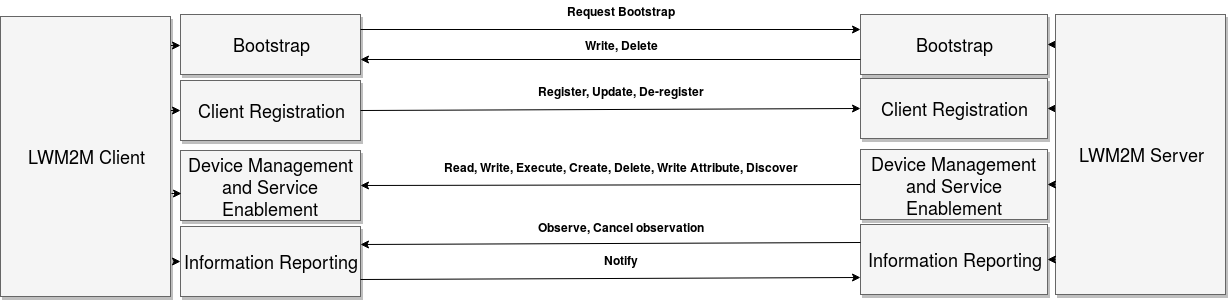
\includegraphics[width=\textwidth]{images/LWM2M-Interfaces}
		\caption{LWM2M Interfaces}
		\label{fig:LWM2MInterfaces}
	\end{center}
\end{figure}

\subsection{World-wide-web Consortium (W3C) - Web Of Things (WOT)}

Since there are many IOT platforms already existing, it is becoming a big problem for developers creating applications that span them. The solution W3C proposes aims to enable worldwide discovery and interoperability by exposing these platforms through the Web with a new class of webservers that support an open framework for the WOT as pictured on ~\ref{fig:WOTWebservers}. In other words, WOT aims to interconnect existing IOT platforms and complement available standards, to reduce cost and risk, and to boost market opportunities.

\begin{figure}[ht]
	\begin{center}
		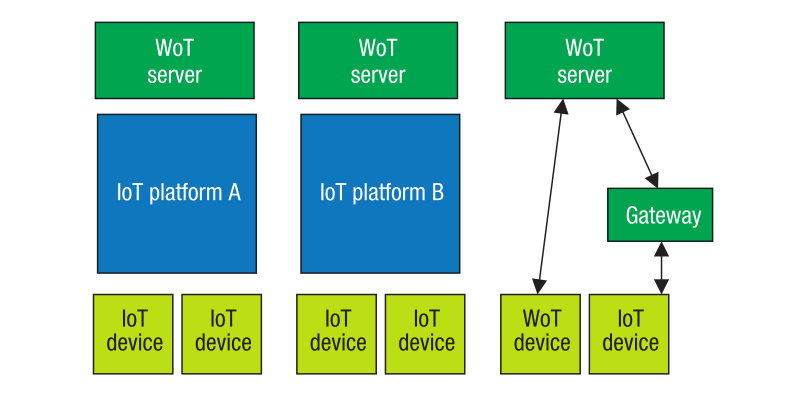
\includegraphics[width=\textwidth]{images/WOTWebservers}
		\caption{WOT framework that bridges the multiple existing IOT platforms}
		\label{fig:WOTWebservers}
	\end{center}
\end{figure}

In W3C WOT all things (devices) are modeled as events, properties and actions, while also possessing metadata describing location of the device, serial number and similar. Firstly, events represent notifications from device to server, such as "battery low" or "the door just opened". Secondly, properties represent information that can be checked through server, such as the temperature or the state of the light switch (on or off). Finally, actions represent commands to coming from server to the device, such as "move the crane from position x to position y" or "turn off". In order to retrieve matadata for things, WOT uses JavaScript Object Notation for Linked Data (JSON-LD).

Analogous to the role played by the Internet as an abstraction layer for networks and networking technologies, WOT describes an abstraction layer over heterogeneous IOT standards, communication patterns, protocols and data formats. This abstraction layer is pictured on figure ~\ref{fig:WOT}, where applications interact with software objects for things (devices, either virtual or physical). Webservers providing this abstraction can be placed on the edge of the network (or in the fog or cloud) to provide efficiency.

\begin{figure}[ht]
	\begin{center}
		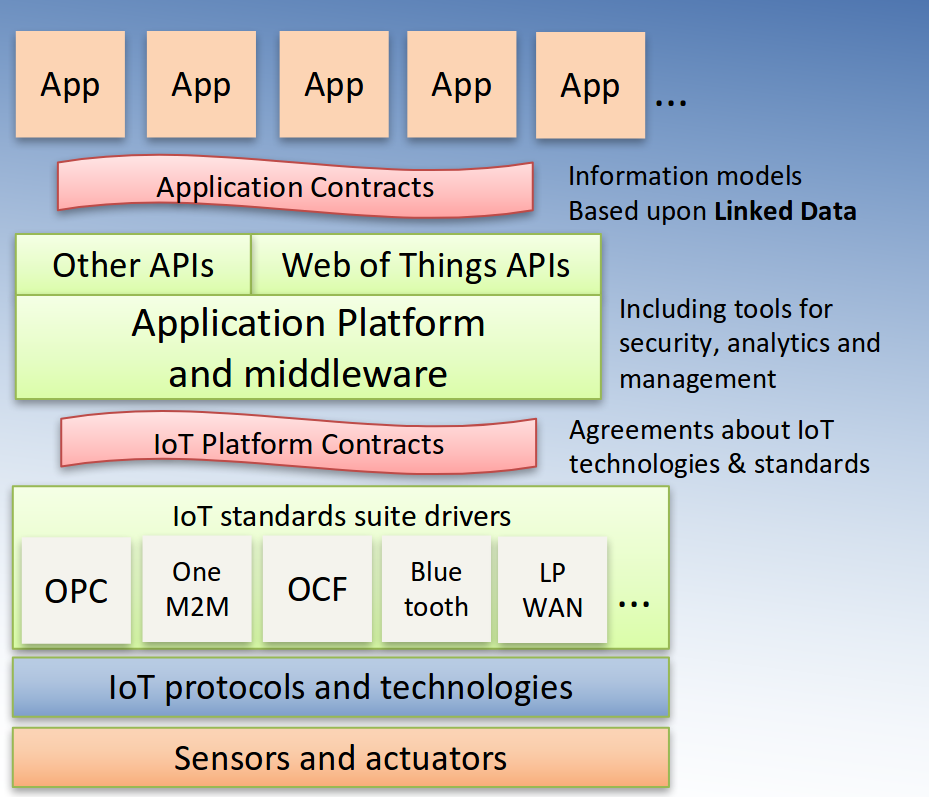
\includegraphics[width=\textwidth]{images/WOT}
		\caption{WOT abstraction layer}
		\label{fig:WOT}
	\end{center}
\end{figure}

Regarding security, WOT is building upon existing security standards such as IOT security foundation, and IOT platforms such as oneM2M (described in section ~\ref{section:Standardization}), claiming to provide end to end security. 

W3C WOT is a new standard, with the working group formed in the beginning of 2017. Since it is a new standard, their work has mostly been abstract, without any real implementations. It is relatively heavy weight compared to LWM2M standard, and focuses on providing a bridge between different platforms unlike LWM2M, that proposes a new solution not necessarily compatible with other existing solutions. Because the work on WOT is in a very early phase and reasons described above I have chosen to make use of LWM2M standard for this thesis.

\section{Policy Based Communications for 5G Mobile with Customer Edge Switching}
\label{CES}

Particularly interesting work by \cite{Kantola} proposes a policy based communication with built in security, while also addressing classical weaknesses of Internet, namely, address spoofing, unwanted traffic and DoS attacks. It is based on a principle that before establishing communication between two hosts (or networks) they need to negotiate interests, and only if they are matching communication is established. These interests are described with a policy.

This work proposes to replace Network Address Translator (NAT) from the edge of the network with their own Customer Edge Switch (CES) node. This node will act exactly like NAT if the sender, who is behind a CES node, is interacting with a receiver using legacy ip. On the other hand, if the situation is reversed CES node will act as a \emph{realm gateway}. Only if both actors are behind CES node it will act as a cooperative firewall negotiating interests of sender and receiver. Because of this, CES can be applied one network at a time making it suitable for IIOT purposes, where vertical fragmentation is a big issue.

Furthermore, CES allows efficient communication by dropping unwanted traffic at the edge and in that way reducing amount of traffic that passes trough network. Also, CES makes use of Domain Name Servers (DNS) to find receivers faster using Fully Qualified Domain Names (FQDN) and MS-ISDN numbers.

In essence, policy database holds all policies and can be accessed through API. Before communication is established, policies of both actors are checked and if they match communication is allowed. Example is shown on ~\ref{fig:PolicyBasedCommunicationExample}.

\begin{figure}[ht]
	\begin{center}
		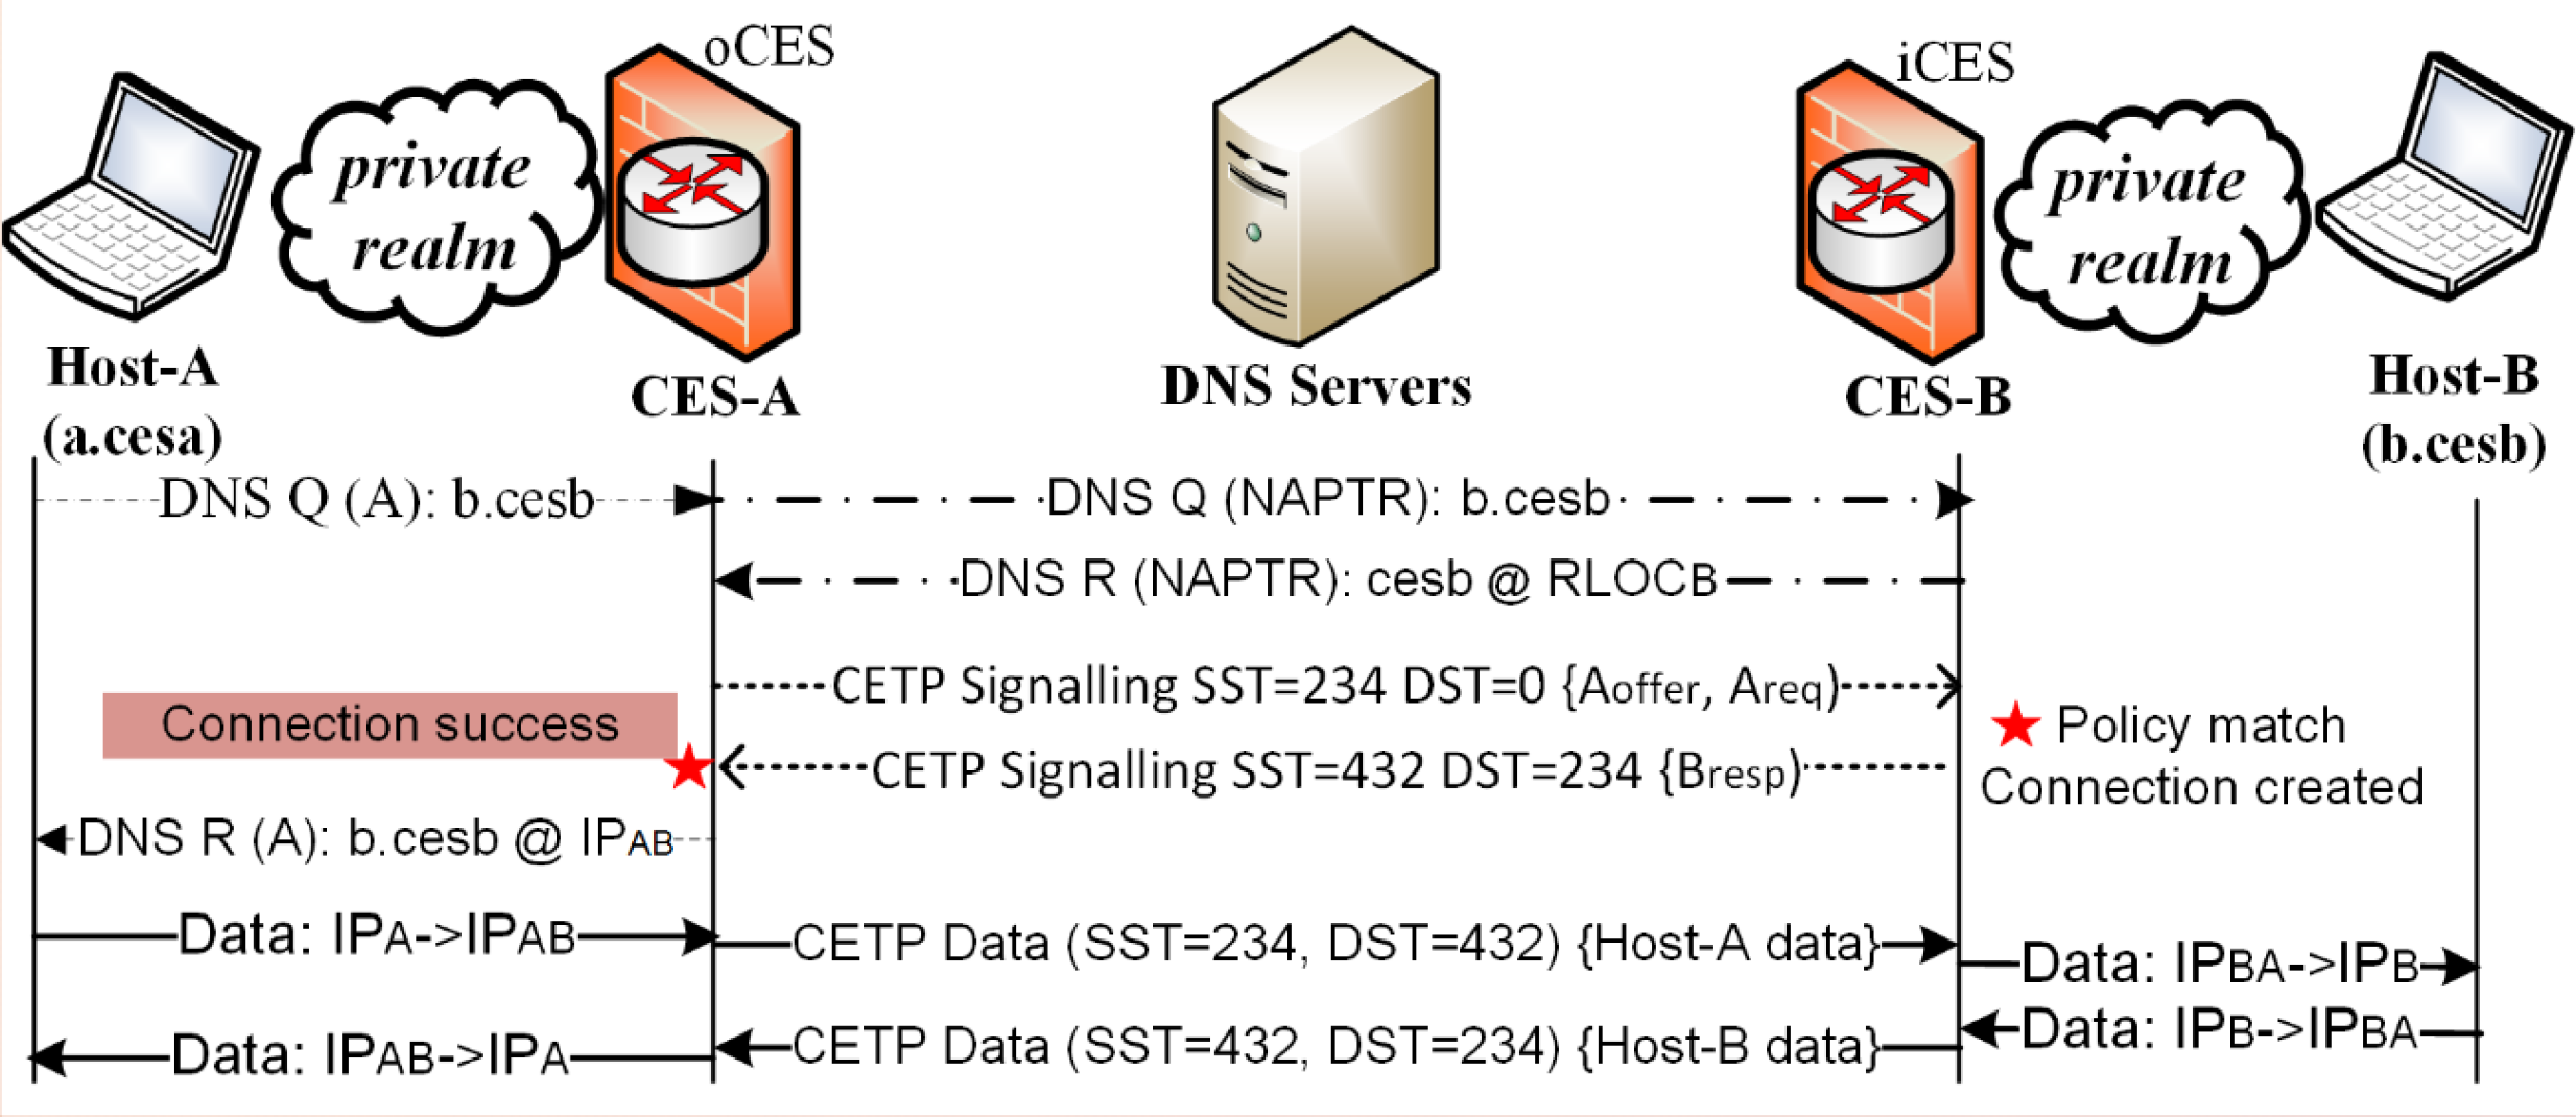
\includegraphics[width=\textwidth]{images/PolicyBasedCommunicationExample}
		\caption{CES communication example}
		\label{fig:PolicyBasedCommunicationExample}
	\end{center}
\end{figure}


\chapter{Requirements}
\label{chapter:requirements}

To design a solution, environment around the problem needs to be understood, specifically, stakeholders involved and what needs they have. This chapter explains several industrial use cases with aim to familiarize the reader with environment Contracting Service is tailored for, followed by concrete requirements of this solution. Since there are countless number of different use cases, not everything can be covered, especially because new applications are continuously emerging. Therefore, this solution needs to be flexible to cover most of the existing and future use cases.  

\section{Context}
\label{section:context}

This section describes three representative industrial use cases in order to help reader understand the range of applications. All use cases have a common core even though they seem very different from each other as it can be seen from the following text.

\subsection{Smart Crane}

KoneCranes have donated a smart crane to Aalto Industrial Campus as a tool for research. This crane is an indoor crane whose head (which carries the load) is mounted on rails allowing it to reach every position inside, crane is pictured on figure ~\ref{fig:KoneCranes-CraneK16052}. Following information was gathered through interviews with researchers and with KoneCranes and it will be used as a representative example for the rest of this work.

\begin{figure}[ht]
	\begin{center}
		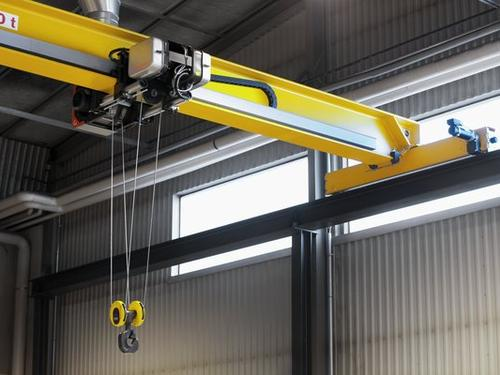
\includegraphics[width=\textwidth]{images/KoneCranes-CraneK16052}
		\caption{KoneCranes Indoor Crane (model K16052)}
		\label{fig:KoneCranes-CraneK16052}
	\end{center}
\end{figure}

This crane has many sensors attached to make it automated and smart as possible. These sensors
bring many features, namely {\bf load weighting} (which can also be used to detect
whether the crane is stuck somewhere), {\bf remote monitoring } of the position of the crane,
{\bf signaling} when some error or warning has occurred, {\bf live video feed } from camera attached
above the hook (at the moment, not used for automation but could be supported in the future,
for example, image processing to detect obstructions) and more.

There are multiple stakeholders in this ecosystem and all of them require some of the data
that Crane generates, although not all information should be available to them, only
the bare minimum that is required by their business. These stakeholders are KoneCranes, 
maintenance service (part of the KoneCranes) and users of the crane. Currently, KoneCranes has access to all the data Crane generates, but in order to 
increase security, this should not be the case.

\subsubsection{Maintenance}

Maintenance service makes use of usage data (alarms, usage parameters) to monitor and predict maintenance needs of the cranes. They also use the data together with the customer, in order to review their maintenance spend of the assets, study patterns to reveal relationships between variables and more. Following are some of the examples of use cases.

One part of the crane that needs to be changed most often are the breaks.
Breaks have limited number of uses and this number is approximately known
(there is a regulation in place that requires brakes to be changed regularly).
In order to determine whether the breaks needs changing or repair, maintenance service requires information about their usage. This information is provided by a pressure sensor installed on the breaks. How much pressure is needed to make the crane head stop is directly proportional to weight the crane is carrying which can then be used to calculate the wear of the breaks.

Large and expensive machines like this crane are under warranties and in order to determine whether the warranty is valid, maintenance service needs to know if the crane has been used in a proper way. Therefore, they need information coming from different sensors installed on the crane. These sensors include: 

\begin{enumerate}
	\setlength{\itemsep}{1pt}
	\item Pressure sensor on the crane head: determining whether the weight carried is in the recommended limits.  
	\item Temperature sensor on rails: when the crane head moves on the rails, friction generates heat and heat levels needs to be in a recommended limits in order for warranty to be valid.
	\item Pressure sensor on rails: determining whether they have been properly oiled.
	\item Humidity sensor: which determines whether the crane is kept in an environment suitable for it.
	\item Speed sensor: which determines whether the speed of crane head does not exceed recommended limits.
\end{enumerate}

Sensors listed are just several examples, and they can provide enough information for maintenance companies to determine whether the crane is being properly used. Crane sensors can also 
detect some irregularities and issue a warning (or error) directly to maintenance companies so that the problem can be addressed as fast as possible. 

Information like this should be disclosed to the maintenance service, while
restricting the access to data that can be used to infer the processes inside the factory. Examples include, position of the crane in a certain
point in time, or live feed from the camera mounted on the head.

\subsubsection{Users of the Crane}

Inside a factory there are different actors with different privileges. These actors can be roughly grouped in two categories: workers and managers. 
Worker operating the crane should have restricted access to data the crane operates. Information that he needs is tied to the current operation of the crane and some of the sensors that give that information are following. Position sensor, which tells him where the head of the crane is in space, and pressure sensor measuring the weight of the load. On the other hand, worker should not have information about the conditions of the brakes or temperature of the rails since it is of no use to him.

Managers responsible for multiple workers and machines should have access to all information related to operations of these machines. In that way, they can monitor their workers remotely, ensuring that everything is operating smoothly.

In the future, machine to machine communication will be utilized much more, for example, 
in a setting with two Cranes operating (automated, not by human) in the same room they 
should be able to signal to each other with their planned path in order to avoid collisions
and to optimize the process. In this way, need for a centralized control is eliminated (or at
least minimized).

\subsubsection{KoneCranes}

KoneCranes needs access to some of the data that Crane generates, in order to make product improvements, react to possible reliability problems and get better specification for new product generations, and adjust warranties.
They analyze all types of data that Crane generates including: 

\begin{enumerate}
	\setlength{\itemsep}{1pt}
	\item Manufacturing data: such as component lists and manufacturing dates.
	\item Usage data: including number of hours in operation, weights carried, mileage of the crane head and more
	\item Sensor data: such as vibrations and temperature
	\item Maintenance data: examples include maintenance task history, ordered materials and more.
\end{enumerate}

As mentioned, at the moment KoneCranes has access to all the data Crane generates and their customers are aware
of that. For privacy reasons, and in environment with multiple manufacturers, data access should be restricted to only what is needed for a specific role. 

\subsection{Smart Traffic}

Recently, smart traffic is emerging as promising trend with the idea to automate transportation of goods and people. Big corporations, such as Google, Tesla, Mercedes and Uber have already joined the race with their models but many technological, legal and business obstacles are holding back its deployment. Integration of these vehicles into regular, non-automated traffic is a big challenge since it needs to take into account human error and correct it if possible.

One interesting example are smart convoys, driver-less trucks transporting goods in a convoy. For this to be secure, communication between trucks needs to be in real-time so that all, for example, obstructions noticed by sensors on truck in front are conveyed to the rest in time to react (slowing down or avoiding obstruction). It is also very important that only authorized people have access to data convoy produces, because if something gets tampered with, human lives are at stake along with structural damages. 

For these security reasons not all stakeholders should have access to all the data but only to what is necessary for their operations. Stakeholders involved are: manufacturers; maintenance company; users; and third parties. Firstly, manufacturers should not have access to data that discloses anything that is confidential for truck users, for example, exact location of the convoy in any time because this information can be used to get insight into operations of users. Secondly, manufacturers might not want to give out all information to their users, either because of confidentiality or because it might discredit them. Thirdly, maintenance companies should have only information about the state of the parts of truck. How many times have the breaks been used, level of motor oil, gas and similar, which they need in order to schedule maintenance control. Finally, third parties could be any company, or public, that benefits from data these trucks produce and fit into business models of manufacturers or users. For example, traffic control application that provides information about how many convoys are on a particular road so that if the number is too high, traffic jams are expected.

\subsection{Connected Goods}

The  servitisation  of  physical  goods  will  be  of  strategic  importance  for the  manufacturing  industry, where instead of selling parts and machines it will be possible to sell engine hours, kilometers and similar. The vision here is that goods will remember how they were made and produce data throughout whole cycle of their usage, even giving insights into customer satisfaction with those goods. In this case, privacy is a big obstacle, because it is hard to assure customer that data you collected in their home or workspace is not going to be used by anybody they do not want to.

Consider a scenario where all goods in your apartment from carton of milk to air-conditioning are equipped with sensors. Milk carton might posses a heat sensor, which alerts when milk is being kept in a warm place for too long, labeling it as spoiled and ordering fresh one from a local marketplace. Same data can be used for statistical purposes by a third party, to determine, for example, how much milk is being wasted by a nation and use it to adjust size of milk cartons or predict peaks in milk consumption. With some more complex goods, such as air-conditioning, predictive maintenance can be realized with sensors that tell if a particular part is wearing off and alert maintenance service specified by user or manufacturer of that machine. Subset of the data generated by air-conditioning can be used by health organizations to determine whether people are living in unhealthy environments, for example, by checking the ratio between how many times air filters have been changed over hours of usage.

Scenarios described in previous paragraph are just few out of many possible ones and it is impossible to tell, which ones will be implemented. Although, we have to prepare for the future by designing a flexible system that can withstand rapid changes in the ecosystem.

\section{Contracting Service Requirements}

At this point, the environment Contracting Service is tailored for has been explained. It is clear from previous section that this solution requires different accounts for all actors involved according to their role. These roles are, roughly, be divided into three groups: Administrators, Manufacturers and Customers.

Remainder of this section is organized into four subsections. First subsection will give general requirements for this platform, spanning requirements regarding security, user interface design rules and functional requirements required for all roles. Following subsections will describe requirements for each role in the system, administrator, manufacturer and customer respectively.    

\subsection{General Requirements}

Following text will describe general requirements for this solution, drawn from the context explained in section ~\ref{section:context}. It will address requirements related to security, user experience and functional requirements not tied to any specific role.

\subsubsection{Security}
\fixme{Talk about general security especially of devices,Authentication}
\fixme{talk about most common attacks, like cross site request forgery}


\subsubsection{User Experience}
\fixme{ Niemens 10 rules of good design?}

\subsubsection{Functional Requirements}
\fixme{, some stuff like changing user info, checking user info, managing devices/policies for device or set of devices/machine }

\subsection{Administrator Requirements}

Administrator of the platform has the simplest role in the system, although he has big responsibility. He is a central, impartial authority that makes sure that the system is running smoothly. Apart from regular responsibilities of system administrator, he is \emph{required to create accounts for manufacturers} and manage them. 

This requirements comes from the fact that, in order to qualify as a manufacturer, you need to have a verified manufacturing company. In order to fully understand the need for this requirement, consider a scenario where everybody is allowed to create an account and pose as a manufacturer. This scenario introduces security concerns, such as a party acting as a manufacturer and assigning fictional devices to a customer, thus affecting customers view of the platform.

\subsection{Manufacturer Requirements}

Manufacturers of smart industrial machines have a central role in the whole ecosystem, they are the providers of the service of selling or lending machines. Therefore, their requirements are of great importance. They have all necessary information about machines they are manufacturing, thus, they should be the ones adding the machines to the system and assigning them to the customers. Following list will explain all of their requirements thoroughly:

\begin{enumerate}
	\setlength{\itemsep}{1pt}
	\item \textbf{\textit{Create customer accounts}}: Allowing anybody to create a customer account may create many empty accounts that are only taking space in the database. Furthermore, there is no use for them if they do not possess any machines. Therefore, when customers buy or lend a machine \emph{for the first time}, their accounts need to be created. Depending on the needs of the customer, opening multiple accounts should be possible. 

	\item \textbf{\textit{Managing templates}}: Almost every machine that is being produced is not one of a kind, it is made following a model. Manufacturers offer many different models to their customers, such as a smart crane pictured on figure ~\ref{fig:KoneCranes-CraneK16052} with model number K16052. Therefore, manufacturers need a way to define templates describing different models of their machines. These templates represent a simplified "digital twin" of a particular machine describing devices that are attached to it. This requirement consists of three smaller requirements:

	\begin{enumerate}
		\item \textbf{\textit{Add templates}}: Way to introduce new templates needs to be available.
		\item \textbf{\textit{Delete templates}}: Deleting faulty or outdated templates needs to be available.
		\item \textbf{\textit{View templates}}: Overview of all templates needs to be presented to manufacturer. 
	\end{enumerate}

	\item \textbf{\textit{Add machine through a template}}: When the necessary templates are added to the system, manufacturers should be able to instantiate them to create a machine and add it to the system. Adding machines following a template reduces error and work needed when inputing data for all devices for a machine.

	\item \textbf{\textit{Add custom machines}}: As mentioned in Managing templates, almost every machine is made using a template. Although, some machines are custom made on a request of the customer. These machines do not require a template because they are not being massively produced. Therefore, a way to add custom machines is required.

	\item \textbf{\textit{Remove and modify machines}}: For any machine, regardless of how it was inputed into system, there needs to be a way to remove them or to modify their contents.

	\item \textbf{\textit{Manage machines and devices}}: When all necessary machines are added to the system they need to be assigned to customers. It should only be possible to assign machines to the customers of a specific manufacturer (not the customers of different manufacturers). This requirement consists of three smaller requirements:
		\begin{enumerate}
			\item \textbf{\textit{Assign machine or device to customer}}: A way to assign a certain machine or device so it becomes visible to the customer needs to be available to the manufacturer.
			\item \textbf{\textit{Remove assignment of machine or device}}: Reverting the action of assigning a machine or device to customer needs to be provided in order to account for faulty assignments, or if the machine or device was lent for a certain period of time.
			\item \textbf{\textit{View assignments}}: In order to control which machines and devices are assigned to whom, an overview of assignments needs to be provided.
		\end{enumerate}
\end{enumerate}

\subsection{Customer Requirements}

Customer requirements are slightly more complicated that manufacturers. Only one account (or a fixed number) of accounts is not necessarily sufficient since the buyer of the machine is rarely the user of the machine. Inside every company there is a hierarchy of responsibilities, where different people are responsible for a subset of machines that the customer company owns. Therefore, it is necessary for customer to be able to create as many accounts as his business requires (this number can be zero). These accounts that a customer creates shall be referred as users in the remainder of this thesis. Following text will list customer requirements, followed by requirements that user shares with customer:

\begin{enumerate}
	\setlength{\itemsep}{1pt}
	\item \textbf{\textit{Create user accounts}}: As mentioned above, creation of user accounts is crucial in order to assign responsibilities for certain machines to several actors inside a company. These actors are some type of managers overlooking the machines they are responsible for.

	\item \textbf{\textit{Manage machines and devices}}: When all necessary machines are added to the system by manufacturers and assigned to customers, they need to be assigned to users responsible for them. In certain cases (for example, in a small company), customer retains all responsibility for machines and do not assign them to anyone else. This requirement consists of three smaller requirements:
		\begin{enumerate}
			\item \textbf{\textit{Assign machine or device to user}}: A way to assign a certain machine or device to the user needs to be available in order for the user to manage access to the machine or device.
			\item \textbf{\textit{Remove assignment of machine or device}}: Reverting the action of assigning a machine or device to the user needs to be provided in order to account for faulty assignments, or if the machine or device needs to be assigned to someone else.
			\item \textbf{\textit{View assignments}}: In order to control what machines or devices are assigned to whom, an overview of assignments needs to be provided.
		\end{enumerate}
\end{enumerate}

Requirements listed above are only for the customer. User requirements are similar to customer with the exception of creating additional accounts and assigning machines. Following list describes additional requirements of customers which are also all requirements of users:

\begin{enumerate}
	\setlength{\itemsep}{1pt}
	\item \textbf{\textit{Allow access to machine or device}}: Allowing customers to define who can access the data their machines produce is highly important. Customer should be able to define access for the whole machine or parts of the machine by controlling access to particular devices, such as a temperature sensor on crane previously described in section ~\ref{section:context}. Additionally, customer needs to be able to define duration and direction of the communication, explained bellow:
		\begin{itemize}
			\item \textbf{\textit{Duration}}: Duration of allowed access is defined by start and end date.
			\item \textbf{\textit{Direction of communication}}: Communication from customer device to the target means that only customer device can send data to the target while rejecting all requests from the target. Opposite direction means that the target can only send requests to the customer device, such request typically give instructions to the device. Allowing flexibility to define direction of communication is highly important to the customer.
		\end{itemize}

	\item \textbf{\textit{Remove previously allowed access to machine or device}}: A way to revert action of allowing access to a machine or device needs to be provided. 
		
	\item \textbf{\textit{View who has access to your machines}}: In order for customer to be fully aware of who has access to their machines, and overview needs to be provided.

\end{enumerate}



\chapter{Prototype Implementation}
\label{chapter:implementation}

For the implementation of contracting service I have used Django framework because it is powerful but also easy to use, and it provides a fixed structure to organize the project. Django framework provides built-in modules for most of the common functionalities with a good security architecture. Along with Django, I have used Bootstrap for styling since it is light-weight and simple.

In this chapter, I will present a brief description of technologies that I used followed by a brief overview of the whole project, showing how different parts fit together before digging into details.

\section{Technologies Used}

In the following text, I will describe two technologies that were used for this implementation in order to give justification of why they are a perfect fit for this project.

\subsection{Django Framework}

Django is a high-level Python Web framework that unlike a library, forces a structure to separate concerns and encourage rapid development and clean, pragmatic design. Structure of Django is influenced by Model-view-controller (MVC), which is a pattern used in software architecture for interactive software or application. 

Model maintains the state of the application by holding the data. In web development, that data is stored in a database. Model abstracts the database typically using a Object-relational-mapper (OBM),	 which maps the data to objects (in case of Django, python objects) and vice versa. Model also takes care of any restrictions on data and takes care of validating, making sure that correct data is stored.

Concern of the view is to generate user interface. In web applications, this means producing HTML typically using a \emph{templating language}. Data is acquired from the Model (typically through Controller, which will be explained in further text) and mixed with HTML using templating language. View can format the data to suit the requirements of a particular view. In simple words, view controls what user sees.

Controller, in a simplest interpretation, controls which views to use based on user input and data from the models. In a broader interpretation, it handles business logic, using models and what rules they enforce.

Django Framework uses a variation on the traditional MVC pattern called Model-Template-View (MTV). Firstly, role of the Model is the same as in MVC, where Django abstracts the database using OBM, instead of tables you deal with classes and instances of data as objects. Secondly, the role of View in MVC is represented in Django using Templates and View. View in Django has a slightly different meaning than in MVC, it represents which data needs to be presented to a user, not necessarily how the data looks. Views get user input (HTTP request), then they access necessary models followed by processing of data, if necessary, and pass it to Templates. Role of Templates is to create the final HTML presented to a user using the data from Views. Finally, role of the Controller can be viewed as whole framework and URL-routing. URL-routing is achieved in Django with a simple 'urls.py' file, which links URLs to views.

Django Framework provides built-in solutions for most of the common tasks that almost every website has. Since this work is not about Django Framework I will only cite subset of parts used in this prototype:

\begin{enumerate}
	\setlength{\itemsep}{1pt}
	\item User management: including creating users, authenticating users, creating sessions, managing cookies, managing user groups and more.
	\item Security mechanisms: in order to prevent most common forms of cyberattacks such is cross-site request forgery.
	\item Support for number of email back-ends.
	\item Efficient mechanism for creating forms from Models.
	\item Creating custom decorators to provide authorization for certain groups of users to a view.
\end{enumerate}

Most importantly, Django Framework has an enormous user base and excellent documentation making it very comfortable to work with. Having a big user base means that most of the questions you might have are already answered and easily accessible. These are the reasons I have chosen Django for this so lution.

\subsection{Bootstrap}

Bootstrap is an open source toolkit for developing with HTML, CSS, and JS. It is very light weight and perfect for applications that do not require a lot of styling. Bootstrap library is easily included in Django templates using just a \verb!<link>! HTML tag.

Bootstrap library is only one CSS file providing many different classes for styling appealing to human visual cues (for example, red for danger, blue for default and more). It relies on a twelve column system for layout, which, if used correctly, brings responsiveness (for different screen sized) on its own. Bootstrap has a big community of users who share snippets of their code providing different functionalities fulfilling almost any need in modern web development.

\section{Overview}

This solution is a Web platform for managing small devices and controlling who has access to the data they generate. Most challenging part was understanding the users of the platform and their needs. Following section describes account types, which correspond to roles they have, followed by the brief description of main parts of the platform.

\subsection{Account Types}

In the Industrial Internet context, I have identified four different types of accounts, with their separate views of the platform depending on their role. Views of these accounts have a common core although they are suited for different purposes. 

Firstly, there needs to be a central authority that distributes accounts to verified manufacturers of industrial machines. In order to receive manufacturer account you need to contact this central authority, which could be a standardization agency but it can be any impartial actor. When that authority verifies that your company is who they claim to be, several accounts can be issued depending on the number of departments that company has or any other criteria depending on the agreement with the manufacturer company. Since the only responsibility this authority has is creating accounts for manufacturers I have used standard Django admin page (and admin account) for its implementation, stripped down to only basic functionality for managing accounts.

Secondly, manufacturers account is assigned to companies that produce smart machines. Their responsibility is to add devices (and update their information if necessary) to platform and assign them to machines (detailed description of devices will be given in subsection ~\ref{deviceManagement}), which are abstract representation of real machine (such is a smart crane) and devices it possess. When the machine has been bought by the customer, manufacturer creates an account for customer (in case they do not possess one) and assigns it to them, giving them full control over who can communicate with that machine. In a case where a customer already has an account, it is customers responsibility to "subscribe" to manufacturer in order for manufacturer to see their account, this is done through a simple form which will be described in section ~\ref{section:customer}. Manufacturer account will be described in detail in section ~\ref{Manufacturer}.

Thirdly, customer account is assigned to owners of the smart machines. Their view is restricted to only devices and machines that they possess and they can manage policies (control access to devices) for those devices only. Along with the possibility of managing policies, customer account can create multiple user accounts (which represents people responsible for single machines or group of them) and assign machines or devices to them. In this way, customer account has a full overview of what policies are in place and who created them while also being able to add or remove faulty ones or general ones (like allowing customers work computer to access all the data or opening their data to a statistical agency). By being able to create user accounts customer can pass on the responsibility and fine tuning of policies for certain machines down the hierarchy of the company.

Finally, user account is assigned to people responsible for a subset of machines that a customer company possess. These accounts are restricted to only managing policies of the machines assigned to them without the possibility to create more accounts or manage devices in the system. Overview of accounts and their views are visualized in figure ~\ref{fig:accountTypes}.

\begin{figure}[ht]
	\begin{center}
		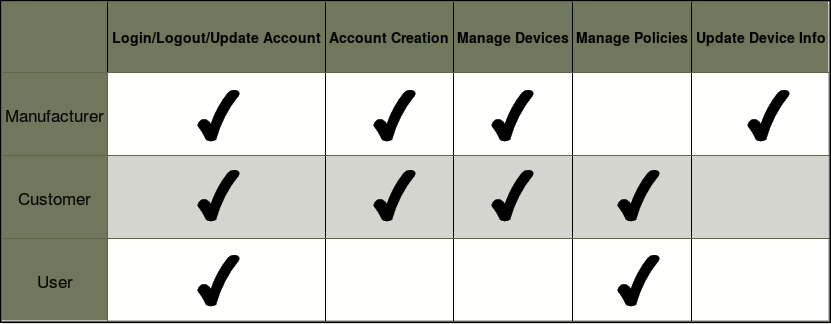
\includegraphics[width=\textwidth]{images/Functionalities}
		\caption{Account types and their views}
		\label{fig:accountTypes}
	\end{center}
\end{figure}

\subsection{Device Management}
\label{deviceManagement}

As previously mentioned, manufacturers task is to add devices to the system, filling all necessary information about the device defined by LWM2M standard described in ~\ref{section:LWM2M}. This information consists of manufacturer name, model number, serial number, public key or identity of the device along with a descriptive name used to refer to it in the system. Public key or identity according to LWM2M standard could be a certificate, a pre-shared key, raw public key or nothing. Since all these, except last one, are similar and exist in standard only to provide flexibility for the manufacturers, only pre-shared key is supported in this solution, although it can easily be extended. 

Further following LWM2M standard, which has a client-server architecture, devices act as a client where my solution acts as a bootstrap server. When a device gets connected to a network, it communicates its IP address (in a form of IPv4 or IPv6) and FQDN or MSISDN to a bootstrap server which saves it for use when managing policies. Example of information implanted on a device is shown on figure ~\ref{fig:device}.

\begin{figure}[ht]
	\begin{center}
		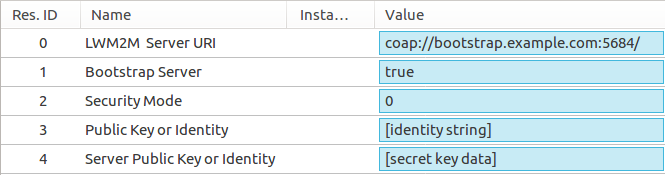
\includegraphics[width=\textwidth]{images/Device}
		\caption{Example device}
		\label{fig:device}
	\end{center}
\end{figure}

Server URI represents the URI of my server, which enables a device to locate it. Only after the server has verified identity of the device, using pre-shared key, it can store devices IP address. In an event when a device is moved to another network (changing its IP address), a device communicates a new IP address which replaces the old one and all policies get updated with a new address.

\subsection{Policy Management}
\label{policyManagement}

Work described in section ~\ref{CES} is very extensive and is made with mobile communications in mind. Although, the idea of policy based communications is perfectly suitable for these purposes since allowing communication between a device and some host can be done in one simple HTTP request to Policy Database. Policy Database holds all policies describing who is allowed to communicate with whom. This database could be distributed or in one central place, although that is outside of the scope of this work, but it has one API that hides the way database is arranged and is the only way database can be accessed. 

Only four different API requests are used in this work. These requests are for inserting, deleting, retrieving and updating firewall policies using Http Post for inserting and deleting, Http get for retrieving and Http put for updating. Inserting policies require following information and they are sufficient for the CES node to determine whether the communication should be established, whether the package should be dropped at the edge: 

\begin{enumerate}
	\setlength{\itemsep}{1pt}
	\item Target IP address and port - target represents a host wanting to communicate with a device.
	\item Source IP address and port - representing a device, extracted from a database in my system.
	\item Start and end of validity timestamps - allowing scheduling of access to devices.
	\item Direction of communication - representing, whether only reporting of data from the device to the host is allowed, sending data to a device or both.
	\item Transport protocol - in this case CoAP is used, justification is provided in section ~\ref{section:LWM2M}.
	\item FQDN or MSISDN - helps speed up the search for receivers as mentioned in section ~\ref{CES} and is used for querying policies.
\end{enumerate}

Direction of communication can be bi-directional or uni-directional (from host to device, or device to host). Bi-directional communication is a regular case, when a host sends a request to a device and gets data or acknowledgment in return. Uni-directional communication is useful in cases where the devices just need to send data (for example, temperature readings) to some external host who is subscribed to them, without a possibility of that host controlling the device (for example, sending request for shutdown). Other way around, uni-directional communication from host to a device could be useful in rare cases where a host is allowed to request from a device to do a task, or send data to some other host. Therefore, all three options are supported in this work.

Deleting and retrieving policies is done using only FQDN or MSISDN (depending on, which one is available for a device), where updating is done the same way as for inserting only different HTTP verb is used. Graphical interface for managing policies will be described in the remainder of this section where all views from different accounts are explained.

\section{Manufacturer}
\label{Manufacturer}

When manufacturer creates session by logging-in to the platform he is directed to a home page. Home page for manufacturers contains (along with navigation bar, which is always present) only a simple form to create customer account pictured on figure ~\ref{fig:CreateCustomer}. This form, along with most of the forms in this solution, is created using Django ModelForm which created a form using database model of a user. When the form is submitted, customer account is made inactive and an automatic email is sent to the provided email address for verification. Automated emails are realized in this prototype using django built-in wrapper for python smtplib module, using a google email account. Only after the customer follows the link in the email, their account is made active and they are prompted to change their password and provide additional information using update form pictured on figure ~\ref{fig:UpdateAccount}. Update account form is available to all types of accounts, to encourage password change in order to promote security.

%TODO: Merge these two in one
\begin{figure}
	\begin{center}
		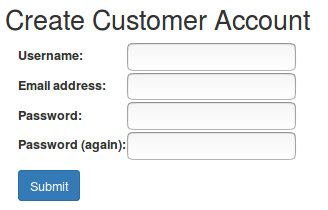
\includegraphics[width=0.4\textwidth]{images/implementation/CreateCustomer}
		\caption{Create Customer}
		\label{fig:CreateCustomer}
	\end{center}
\end{figure}

\begin{figure}[ht]
	\begin{center}
		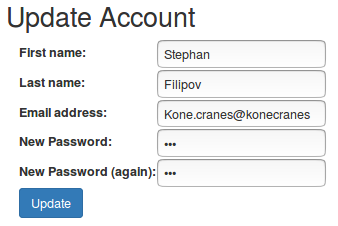
\includegraphics[width=0.4\textwidth]{images/implementation/UpdateAccount}
		\caption{Update Account}
		\label{fig:UpdateAccount}
	\end{center}
\end{figure}

As previously mentioned, manufacturers task is to add devices to platform, which they can later assign to customers that have bought them. Adding of devices is made available in two ways: through "Manage Devices" for custom made machines, or following a previously defined template. For the custom machines, first a machine needs to be created. Machine is an abstract concept that only has a name, which is used to organize devices. For example, AaltoCrane could be a machine and all sensors and actuators that are mounted on that crane are assigned to it. In the process of adding a device to the platform, a machine it belongs to needs to be specified. Note that in order to remove a machine from platform, its name needs to be typed in the text box to prevent accidental removal of machines. Two forms needed to complete this task are pictured on figure ~\ref{fig:AddMachineDevice}. 

\begin{figure}[ht]
	\begin{center}
		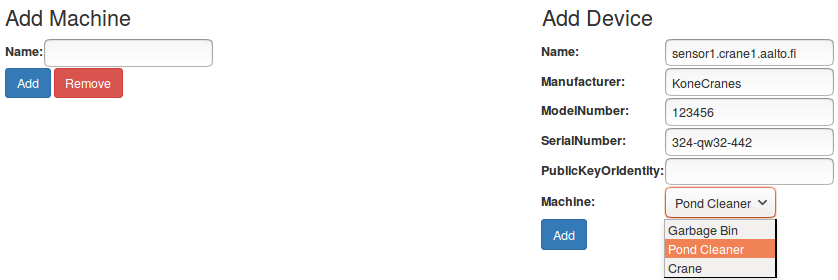
\includegraphics[width=\textwidth]{images/implementation/AddMachineDevice}
		\caption{Adding machines and devices}
		\label{fig:AddMachineDevice}
	\end{center}
\end{figure}

% Mention how templates can be extended in evaluation or future work discussion(mention digital twin)
Other way a manufacturer adds devices is through templates. Templates define how many devices a particular machine that a manufacturer produces has so that when a new machine is created, template can be instantiated to add a new machine. Creation and overview of templates is pictured on figure ~\ref{fig:addTemplate}. 

\begin{figure}[ht]
	\begin{center}
		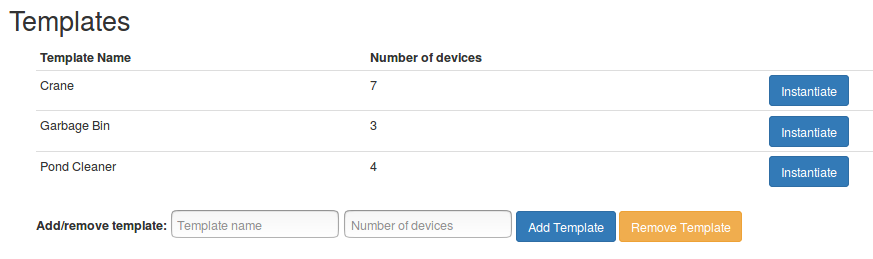
\includegraphics[width=\textwidth]{images/implementation/AddTemplate}
		\caption{Creation and overview of Templates}
		\label{fig:addTemplate}
	\end{center}
\end{figure}

Clicking on the "instantiate" button for a particular machine opens a form bellow. This form asks for the name of the machine (which is supposed to be descriptive, for example Aalto Industrial Campus Crane or similar), and information about devices attached to it. Number of devices in a form is equal to the number defined in the template. Form for a machine with three devices is pictured on figure ~\ref{fig:AddMachineViaTemplate}.

\begin{figure}[ht]
	\begin{center}
		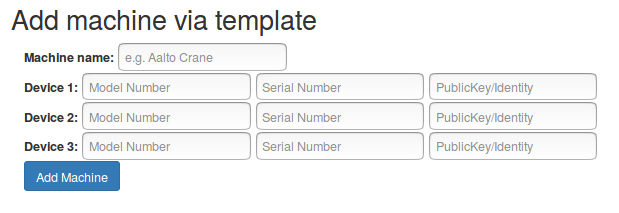
\includegraphics[width=\textwidth]{images/implementation/AddMachineViaTemplate}
		\caption{Instantiating a template with three devices}
		\label{fig:AddMachineViaTemplate}
	\end{center}
\end{figure}

When the customer has an account and all devices are added to the platform and organized to machines, manufacturer needs to assign these devices to customers. Assigning devices to customers can be done on a device level or machine level as pictured on figure ~\ref{fig:ManageDevicesCompany}. No matter if the manufacturer is assigning devices or machines (group of devices) the task is done through a simple form and clicking on an appropriate button, either to add or remove a customer. Removing a customer makes sense in case when a machine or device has been rented or a mistake was made while adding. Removing of devices from a platform is also in a same view because it provides a good overview of which devices are attached to which machines.

\begin{figure}[ht]
	\begin{center}
		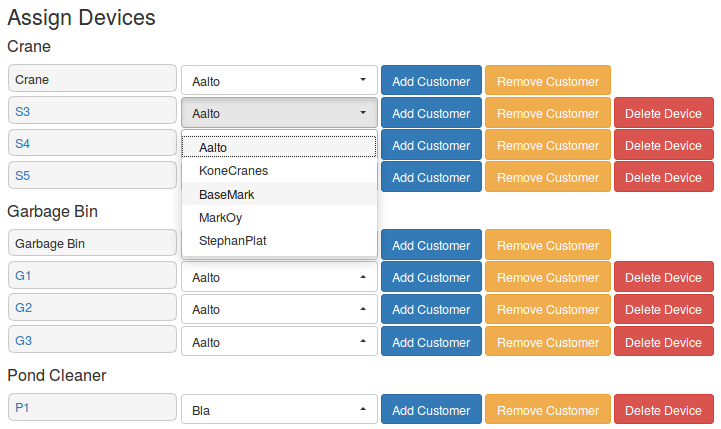
\includegraphics[width=\textwidth]{images/implementation/ManageDevicesCompany}
		\caption{Device Management For Manufacturer}
		\label{fig:ManageDevicesCompany}
	\end{center}
\end{figure}	

In the figure ~\ref{fig:ManageDevicesCompany}, clicking on a device name navigates to a separate page where details about a device can be inspected, and changed if needed as pictured on figure ~\ref{fig:DeviceDetailsUpdate}. Fields in the form are pre-filled with current information about a device, so that typing mistakes or any small changes can be made easily.

\begin{figure}[ht]
	\begin{center}
		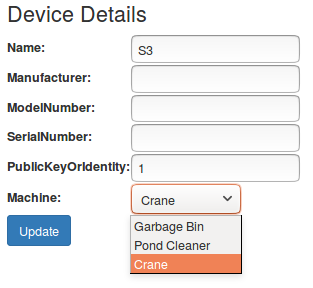
\includegraphics[width=0.4\textwidth]{images/implementation/DeviceDetailsUpdate}
		\caption{Update Device Information}
		\label{fig:DeviceDetailsUpdate}
	\end{center}
\end{figure}

Last element on a Manage Devices page is pictured on figure ~\ref{fig:DeviceAssignment}. This element only provides an overview of which users are assigned to which devices. It is intended to be used along with element pictured on figure ~\ref{fig:ManageDevicesCompany} in order to check whether any mistakes were made and that everything is how it should be.

\begin{figure}[ht]
	\begin{center}
		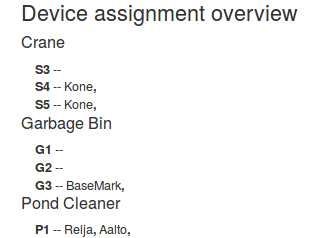
\includegraphics[width=0.4\textwidth]{images/implementation/DeviceAssignment}
		\caption{Device Assignment Overview}
		\label{fig:DeviceAssignment}
	\end{center}
\end{figure}


\section{Customer}
\label{section:customer}

 After logging-in to the platform, customer is directed to a home page where he can create additional user accounts. Creation of user accounts is slightly different from customer accounts as pictured on figure ~\ref{fig:CreateUser}. In the form, for convenience sake, customer can assign devices to a user while creating the account using a multiple choice select field. In case when the account is created for just one device or a small set of devices, this can greatly reduce the number of clicks and queries to the database to complete a task. As with customer accounts, user accounts also need email verification.

\begin{figure}[ht]
	\begin{center}
		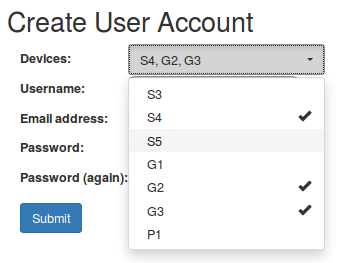
\includegraphics[width=0.6\textwidth]{images/implementation/CreateUser}
		\caption{User Account Creation}
		\label{fig:CreateUser}
	\end{center}
\end{figure}

One very simple but necessary element pictured on figure ~\ref{fig:SubscribeToManufacturer} allows a customer to subscribe to the manufacturer and in that way be visible to manufacturer when assigning devices. Customer only needs to type the name of the manufacturer (that manufacturer communicated to customer in the process of buying the machine) and submit.

\begin{figure}[ht]
	\begin{center}
		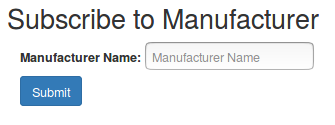
\includegraphics[width=0.6\textwidth]{images/implementation/SubscribeToManufacturer}
		\caption{Inform Manufacturer that you are a customer}
		\label{fig:SubscribeToManufacturer}
	\end{center}
\end{figure}

On "Device Management" page, customer can assign devices to users. His view is restricted only to devices that are previously assigned to him by the manufacturer, and choice of users is restricted to the ones he created (which represent users he is responsible for). Interface for doing this resembles one pictured in figure ~\ref{fig:ManageDevicesCompany} with two exceptions: customer is not allowed to change details about devices; and user is not allowed to 
delete devices from the system. In the case when a machine is no longer used (not needed anymore or replaced with a new one), manufacturer needs to be contacted directly in order to remove the machine from platform. This is because customers can not be allowed to add devices, and if they were allowed to remove devices, they could mistakenly remove the device without the possibility of adding it back. In industrial case, these machines are expensive, large and robust, therefore, they do not need to be removed frequently, which is why I opted for this solution.

As previously mentioned, only customers and users are allowed to control who can communicate with their devices and they control that through policies. "Manage Policies" page contains two elements, one for adding policies, other for removing them and to give overview of existing ones. Customer view is restricted to only devices that are assigned to him (as in case of managing devices) and he can add policies to Policy database using a group of forms pictured on figure ~\ref{fig:ManagePolicies}. Customer only needs to specify IP address (both IPv4 and IPv6 supported) of a host, direction of communication (as explained in ~\ref{policyManagement}), start and end date of policy validity, and click on submit policy. By submitting a policy, customer has allowed a host with specified IP address to interact with a device or all devices that are part of a machine.

\begin{figure}[ht]
	\begin{center}
		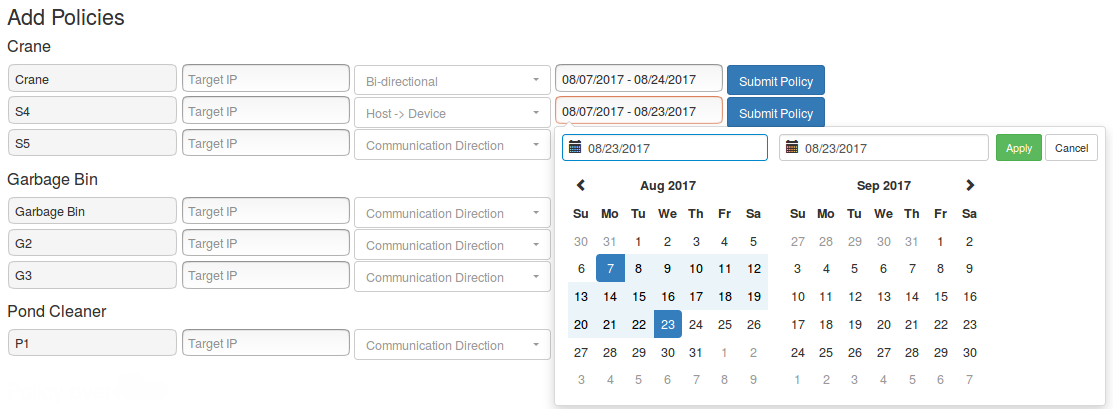
\includegraphics[width=\textwidth]{images/implementation/ManagePolicies}
		\caption{Policy Management}
		\label{fig:ManagePolicies}
	\end{center}
\end{figure}

Second element on a "Manage Policies" page contains overview of all policies related to devices that a customer has. In the same element, customer can remove policies that are mistakenly made or if the circumstances changed since the policy was put in place.

\begin{figure}[ht]
	\begin{center}
		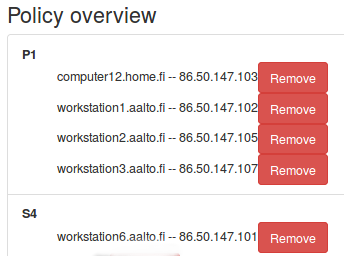
\includegraphics[width=0.6\textwidth]{images/implementation/PolicyOverview}
		\caption{Overview of policies}
		\label{fig:PolicyOverview}
	\end{center}
\end{figure}

\section{User}

Simplest account type is user account. User account can only update information about his account and manage policies for the devices he was assigned to by the customer. "Manage Policies" page for user only contains elements pictured in figures ~\ref{fig:ManagePolicies} and ~\ref{fig:PolicyOverview}.





 
\chapter{Evaluation and Discussion}
\label{chapter:evaluation}

In the requirements chapter, the context for which this thesis is tailored for is described. This context described actors involved and how are they using these machines. From the context, a list of concrete requirements have been drawn and described in the remainder of requirements chapter. Following these requirements, I have implemented a prototype which aims to fulfill these requirements.

In the following sections, I am evaluating the implementation described in chapter ~\ref{chapter:implementation}. Furthermore, I will discuss shortcomings and possible improvements to my solution. This evaluation is done by addressing every requirement described in chapter ~\ref{chapter:requirements}, consequently the current chapter will have similar structure. The general requirements will be addressed, followed by administrator, manufacturer and customer requirements.

\section{Evaluation of General Requirements}

General requirements are not tied to any specific role in the system, they apply to all users. These requirements are grouped into three categories. First group is related to security, second  regarding security, In the following section, requirements regarding security, user experience and functional requirements related to all roles in the system are evaluated. Furthermore, shortcomings are discussed and possible alternate solutions are described.

\subsection{Security}

Securing a web platform is not an easy task. As the security measures are evolving to fill security gaps, new methods on how to breach them are also emerging. Thus, securing a web platform is a process and it constantly needs to be improved. Following list will discuss every security requirement described in section ~\ref{subsubsection:security} and how the implementation has met them:

\begin{enumerate}
	\setlength{\itemsep}{1pt}
	\item \textbf{\textit{Only authenticated users can access platform}}: As previously mentioned in section ~\ref{section:technologiesUsed}, for this implementation a Django Framework was used. Django provides built-in decorator, named @login\_required, to restrict access to certain views. To make sure that only authenticated users can access the platform, every view has been secured with this decorator. 

	\item \textbf{\textit{Platform needs be to robust against common cyberattacks}}: One big advantage of using Django Framework are the built-in protection mechanisms against cyberattacks. Protection against most common cyberattacks is discussed in the following list.

		\begin{enumerate}
		\setlength{\itemsep}{1pt}
		\item \textbf{\textit{Cross-site scripting (XSS)}}: XSS attacks allow a user to inject client side scripts into the browsers of other users. Protection against this is ensured by using django templates, which escape specific characters which are particularly dangerous to HTML. This protection is not completely foolproof since there are cases when it fails. Such examples are well documented in django documentation, and all \verb|<style>| tags used in this implementation are checked against them.

		\item \textbf{\textit{Cross site request forgery (CSRF)}}: CSRF attacks allow a malicious user to execute actions using the credentials of another user without that user's knowledge or consent. CSRF protection works by checking for a secret in each POST request. This ensures that a malicious user can not simply ``replay" a form POST to your website and have another logged in user unwittingly submit that form. Since the malicious user does not know the secret, which is stored in a cookie, he can not execute this request. CSRF protection in django is done by simply putting a {\% csrf\_token \%} tag in every form in a template and securing corresponding view with @csrf\_protect built-in decorator. The {\% csrf\_token \%} creates a hidden input field containing a secret which is then passed to the corresponding view.

		\item \textbf{\textit{Clickjacking}}: Clickjacking is a type of attack where a malicious site wraps another site in a frame. In that way, an unsuspecting user is tricked into performing unintended actions on the target site. In order to protect against this attack, rendering in a frame has been disabled using django X-Frame-Options middleware.

		\item \textbf{\textit{SQL injection}}: SQL injection is a type of attack where a malicious user is able to execute arbitrary SQL code on a database. Such attacks are usually prevented by sanitizing any input coming from an user. Using Django Framework, this is prevented by using querysets and in that way an underlying database driver will escape the resulting SQL. Django also provides developers a way to write raw queries which are vulnerable to SQL injection. In order to prevent SQL injection, raw queries are not used.

		\item \textbf{\textit{Denial of service (DOS)}}: Not much can be done to prevent denial of service attacks at this stage, but rather during deployment of the platform on a server. By not allowing everybody to create accounts on this platform, effect of DOS attack is reduced but it is not eliminated.
		\end{enumerate}

	\item \textbf{\textit{Only authorized people can manipulate machines or devices}}: Django Framework provides support to write custom decorators, to secure access to views on almost any criteria. For this requirement, three different decorators have been made for each account type, namely manufacturer, customer and user. These decorators have been used for each view that belongs to manufacturer, customer or user accordingly. Furthermore, identity of a user is being checked every time a database is contacted in order to make sure that he has required access rights. In the previous point, protection against cyberattacks are discussed, making sure that user identity was not tampered with.

	\item \textbf{\textit{Users personal information can only be changed by them}}: Similar to the previous point, user identity is determined every time user wants to see or change its information. And the validity of their identity is ensured by protecting against common cyberattacks.
\end{enumerate}

Along with security measures described in the list above, HTTPS protocol is used instead of HTTP. This functionality is enabled by configuring Django settings file to redirect all requests over HTTP to HTTPS and also by configuring a server where this platform is hosted.

\subsection{User Experience}

Requirements related to user experience are more of a guidelines than actual requirements, nonetheless, every well designed user interface is following them. Therefore, it is very important that they are satisfied to a logical extent. Following list will briefly discuss how the implementation described in chapter ~\ref{chapter:implementation} has followed Nielsen et. al.~\cite{nielsen199510} ten most important heuristics:

\begin{enumerate}
	\setlength{\itemsep}{1pt}
	\item \textbf{\textit{Visibility of system status}}: For almost every action that user performs, a message informing user about the success of the action is issued in form of a pop-up window. In case of removing a machine (or device) or a template, this message is not issued since the disappearance of the machine or template from the overview is evident.

	\item \textbf{\textit{Match between system and the real world}}: Terms used in the system correspond to real world terms, few examples include a machine, device, manufacturer and customer. 

	\item \textbf{\textit{User control and freedom}}: Actions available in this system are easily reversible, such actions include adding a machine, submitting a policy, and adding a template.

	\item \textbf{\textit{Consistency and standards}}: All terms (such are machine, device, and template) correspond to real world terms and are used consistently throughout the platform.  

	\item \textbf{\textit{Error prevention}}: This requirement is very hard to fulfill, since it is hard to predict kind of mistakes people make. Simple measures are taken in order to prevent mistakes since this platform is not intended for computer illiterate people. Preventing accidental removal of machines and templates is assured by forcing an user to type in the name of the machine or template before deleting them.

	\item \textbf{\textit{Recognition rather than recall}}: Almost all actions in the system require user to select options from the list of available ones instead of typing them in, reducing memory load of the user. Exception are the removal of machine or template because of the reasons described in the previous point.

	\item \textbf{\textit{Flexibility and efficiency of use}}: Tailoring of frequent actions is made available through templates, where manufacturers can simplify the way they add machines in the future by defining a template of a particular machine and instantiating them.

	\item \textbf{\textit{Aesthetic and minimalist design}}: All elements described in chapter ~\ref{chapter:implementation} are necessary to provide desired functionality. Colors and shapes are designed to appeal to human visual cues.

	\item \textbf{\textit{Help users recognize, diagnose, and recover from errors}}: Error messages are presented to a user in plain text, no codes are being used. In order to do so, custom pages for most common http errors are provided. Such errors include ``404 not found'' and ``500 internal server error''.

	\item \textbf{\textit{Help and documentation}}: Home page of the platform, briefly describes how to use the platform.
\end{enumerate}

\subsection{Functional Requirements}

List of functional requirements for all roles is a rather short list, although, still important for this platform to be usable. Following list will describe how my implementation has fulfilled these requirements:

\begin{enumerate}
	\setlength{\itemsep}{1pt}
	\item \textbf{\textit{Users should be able to view their personal information and change it if needed}}: This functionality is provided by using a form shown on figure ~\ref{fig:UpdateAccount}.
	\item \textbf{\textit{Manipulating single devices or all devices attached to a machine in one action}}: Forms shown on figure ~\ref{chapter:evaluation} and ~\ref{chapter:evaluation} allow assigning machines and submitting policies for all devices of a machine or single devices in one action, respectively.
	\item \textbf{\textit{Navigation bar needs to be present}}: Standard navigational bar on the top of the screen, spanning the width of the screen is provided to navigate the website.
\end{enumerate} 

\section{Evaluation of Administrator Requirements}

Administrator of the system has a responsibility to overlook the system and make sure that it operates smoothly. Administrator is required to create manufacturer accounts as mentioned in chapter ~\ref{chapter:requirements}. For the implementation of the administrator view, a django built-in administrator page have been used. This page provides many features, such as managing the user groups, and creating and deleting different types of accounts. For this work, I have reduced functionalities of this page to only be able to manage manufacturer accounts. Managing includes creating, deleting, modifying contents of the manufacturer accounts.

\section{Evaluation of Manufacturer Requirements}

As previously described in chapter ~\ref{chapter:implementation}, manufacturers have their own view of the platform. In the following list, manufacturer requirements are discussed, providing justification on how the implementation is meeting them, while pointing out shortcomings and possible alternate solutions.

\begin{enumerate}
	\setlength{\itemsep}{1pt}
	\item \textbf{\textit{Create customer accounts}}: Fulfilling this requirement was simple. Form pictured on figure ~\ref{fig:CreateCustomer} allows a manufacturer to create customer accounts. Creating multiple accounts with the same username is not possible due to the database restrictions.

	\item \textbf{\textit{Managing templates}}: Only manufacturer account has access to the "Manage Templates" page since they are the only ones who add machines or devices. This was ensured using custom made decorators.

	\begin{enumerate}
		\item \textbf{\textit{Add templates}}: Creating a new template is available through form shown in figure ~\ref{fig:addTemplate}. This is a minimalistic interface which allows the manufacturer to add templates of machines with corresponding number of devices. This solution lacks the sufficient fields to describe the machine. In other words, it is not very expressive, since it only requires information about the name of the machine and number of the devices attached to it. Whereas, real machines are usually comprised of multiple parts and each part has different types of devices attached. It would have been more meaningful to have detailed description of machines, its parts, and types of devices. However, this detailed  description of machines require comprehensive study of "digital twins", which is not the core of this work.

		\item \textbf{\textit{Delete templates}}: Deleting templates is available through same form as for adding templates. Manufacturer is required to input all information about the template and click on a button "delete". It was implemented this way in order to minimize risk of deleting a template by accident.
		\item \textbf{\textit{View templates}}: View of all available templates is also shown on the same figure. For this overview of templates, a table is used.  
	\end{enumerate}

	\item \textbf{\textit{Add machine through a template}}: On a figure ~\ref{fig:addTemplate}, a table with existing templates is shown. In the third column from the left, a button for each template is provided to instantiate a template. Clicking on a button "instantiate" opens a form to add a machine following that template as shown on figure ~\ref{fig:AddMachineViaTemplate}.

	\item \textbf{\textit{Add custom machines}}: Adding custom machines is made available through "manage devices" page through forms shown on figure ~\ref{fig:AddMachineDevice}. These forms are on the "manage devices" page because they do not take much space and they are used frequently when managing devices.

	
	\item \textbf{\textit{Manage machines and devices}}: Managing devices for manufacturer is done through "manage devices" page.
		\begin{enumerate}
			\item \textbf{\textit{Assign machine or device to a customer}}: Assigning machines or devices to a customer is done though forms shown on figure ~\ref{fig:ManageDevicesCompany}. This implementation gives good overview of devices and to what machine are they attached to, although each assignment requires a separate call to the database. Alternate solution that would allow multiple assignments to be done in one call to the database would not give overview of devices. This solution would list all customers and provide a multiple check list to chose which devices to assign to them. Current solution was chosen because it is simpler to use.

			\item \textbf{\textit{Remove assignment of machine or device}}: Removing assignment is done through the same form as for assigning, just by clicking on "remove customer" instead of "add customer".

			\item \textbf{\textit{View assignments}}: Overview of assignments is shown on figure ~\ref{fig:DeviceAssignment}. For each device, assigned customers are listed.
		\end{enumerate}

	\item \textbf{\textit{Remove machines or devices}}: Removing machines from the system is done through the form shown on figure ~\ref{fig:AddMachineDevice}. For the same reason as for removing templates, manufacturer is required to input the name of the machine in order to delete it. Removing devices is done through forms shown on figure ~\ref{fig:ManageDevicesCompany} by clicking on "remove customer" button. Figure ~\ref{fig:ManageDevicesCompany} provides an overview of all devices, thus, this position of the button to remove customer is logical.

	\item \textbf{\textit{Modify machines}}: Modifying machines is done one device at a time. Clicking on a device name in the form shown on figure ~\ref{fig:ManageDevicesCompany} opens a separate page where device information can be changed. 

\end{enumerate}

\section{Evaluation of Customer Requirements}

As mentioned in chapter ~\ref{chapter:requirements}, having only one type of account for customer is not sufficient. Thus, in this work two types of customer accounts are created. These accounts are named customer and user accounts. Customer account is created by manufacturer, and user accounts are created by customer in order to assign responsibilities for different machines down the company hierarchy. In other words, user accounts are created for managers inside the customer company who are responsible for certain machines are people working with those machines. Following text will evaluate and discuss customer requirements arranged in two lists, exclusively customer requirements and requirements related to both customer and user, respectively.

\begin{enumerate}
	\setlength{\itemsep}{1pt}
	\item \textbf{\textit{Create user accounts}}: Creating user accounts is made available to manufacturer through a form shown on figure ~\ref{fig:CreateUser}. This form has been created using Django ModelForm module, which creates forms directly from the models in the database, alike most of the forms used in this implementation. In this case, that model was User.

	\item \textbf{\textit{Manage machines and devices}}: Implementation meets this requirement in a similar way as for the manufacturer. Differences between implementation for manufacturer and customer will be described below:

		\begin{enumerate}
			\item \textbf{\textit{Assign machine or device to user}}: Assigning machines and devices is done through the same form as one shown on figure ~\ref{fig:ManageDevicesCompany}, with two exceptions. These exceptions are: links to access device information and change it are disabled, and buttons to remove devices from the system are removed. Alternate solution for manufacturer view of the same functionality applies in this case too.

			\item \textbf{\textit{Remove assignment of machine or device}}: In order to remove assignment, customer account performs the same action as for assigning, just by using "remove customer" instead of "add customer" button.

			\item \textbf{\textit{View assignments}}: Full overview of assignments for customer is the same as for manufacturer. This overview is shown on figure ~\ref{fig:DeviceAssignment}
		\end{enumerate}
\end{enumerate}

As previously mentioned, above list evaluates and discusses exclusively customer requirements. Following list contains evaluation and discussion of requirements related to both customers and users. 

\begin{enumerate}
	\setlength{\itemsep}{1pt}
	\item \textbf{\textit{Allow access to machine or device}}: Who can access a device is described by a policy as explained in section ~\ref{CES}. Inserting or removing these policies from a policy database allows or denies a certain host to access a particular device. Forms used for manipulating these policies are shown on figure ~\ref{fig:ManagePolicies}. Policies allow high level of customization of the type of access that is allowed, although for this work only required protocol, direction of communication and duration of communication is used.
		\begin{itemize}
			\item \textbf{\textit{Duration}}: In order to define a period of duration of a policy, slightly modified date range picker \footnote{http://www.daterangepicker.com/} is used as shown on figure ~\ref{fig:ManagePolicies}.

			\item \textbf{\textit{Direction of communication}}: All directions of communication are supported. They are defined in select field by choosing appropriate direction (Host -> Device, Device -> Host or Bi-directional).
		\end{itemize}

	\item \textbf{\textit{View who has access to your machines}}: Overview of policies inside a policy database are shown on figure ~\ref{fig:PolicyOverview}.

	\item \textbf{\textit{Remove previously allowed access to machine or device}}: Overview of policies shown on figure ~\ref{fig:PolicyOverview} contains a button to remove a policy.
\end{enumerate}

\chapter{Conclusion}
\label{chapter:conclusion}

This work investigates use cases of smart industrial machines, mostly focusing on the smart crane donated to Aalto Industrial campus, in order to create a contracting service for management of access to smart machines. The research aim of this thesis, defined in section \ref{section:researchQuestion}, is the solution for easy and secure access management for large number of devices in industrial setting. Three sub questions of the research describe the phases necessary in order to answer the main question. These fazes are: gathering and listing requirements of the solution, forming necessary components of the solution and evaluating the solution with respect to requirements. 

Main findings of this work are presented in the chapter \ref{chapter:implementation} showing the necessary components of this solution. Four types of accounts were deemed necessary, Administrator account, Manufacturer account, Customer account, and User account. Administrator has a role to create and manage Manufacturer accounts, since the creation of accounts is not possible for anyone, only for verified Manufacturers. Manufacturer account needs to create Customer accounts on request of customers, add machines and devices to the system and assign them to the customers. Customer account can then either, create User accounts and assign machines or devices to them, or can manipulate access to the machines or devices by inserting or removing policies from the Policy Database. User account has a similar role as a Customer account, only he can not create new accounts or assign devices to other accounts. 

This solution for management of machines and devices have a small scalability issue in terms of user experience. When a large number of devices are added to the system, the overview of machines and devices becomes cluttered. Thus, finding a right machine or device can be problematic. This issue can be solved by including a search option. Search option should take into account number of devices, types of devices or machines, and names of machines or devices. Moreover in terms of performance, increasing number of devices pose some scalability issues when contacting the Policy Database. These issues can be simply solved by distributing the Policy Database on several locations. However, smart ways of distributing the Policy Database is out of the scope of this work.

Implementation described in chapter \ref{chapter:implementation} is constructed according to the requirements described in section \ref{chapter:requirements}. Requirements were extracted from context and grouped into three main categories general requirements, manufacturer requirements and customer requirements. General requirements are further divided into security, user experience and functional requirements related to all roles in the system. These requirements are then evaluated in section \ref{chapter:evaluation}.

Chapter \ref{chapter:background} gives background information about the problem my solution is solving. Firstly, it introduces the Internet of Things (IoT) and then compares it with Industrial Internet of Things (IIoT) in order to highlight the differences in requirements between them. Secondly, it briefly describes issues regarding standardization, security and privacy. Furthermore, current existing solutions are described and their shortcomings highlighted. Finally, most notable standards are described in more detail (LWM2M and W3C WOT), followed by a work by Kantola et. al. \cite{Kantola,5480987} on which this solution relies to provide a desired functionality. 
 

% Load the bibliographic references
% ------------------------------------------------------------------
% You can use several .bib files:
% \bibliography{thesis_sources,ietf_sources}
\bibliography{sources}


% Appendices go here
% ------------------------------------------------------------------
% If you do not have appendices, comment out the following lines
\appendix
\chapter{First appendix}
\label{chapter:first-appendix}

This is the first appendix. You could put some test images or verbose data in an
appendix, if there is too much data to fit in the actual text nicely.

For now, the Aalto logo variants are shown in Figure~\ref{fig:aaltologo}.

\begin{figure}
\begin{center}
\subfigure[In English]{
\includegraphics[width=.8\textwidth]{images/aalto-logo-en}}
\subfigure[Suomeksi]{
\includegraphics[width=.8\textwidth]{images/aalto-logo-fi}}
\subfigure[På svenska]{
\includegraphics[width=.8\textwidth]{images/aalto-logo-se}}
\caption{Aalto logo variants}
\label{fig:aaltologo}
\end{center}
\end{figure}

% End of document!
% ------------------------------------------------------------------
% The LastPage package automatically places a label on the last page.
% That works better than placing a label here manually, because the
% label might not go to the actual last page, if LaTeX needs to place
% floats (that is, figures, tables, and such) to the end of the 
% document.
\end{document}
